\documentclass[11pt,a4paper]{article}
\usepackage[margin=25mm]{geometry}
\usepackage{amsmath,amssymb}
\usepackage{graphicx}
\usepackage{xcolor}
\usepackage{amsthm}
\usepackage{tikz}
\usetikzlibrary{arrows.meta,patterns,positioning}
\usepackage{pgfplots}
\pgfplotsset{compat=1.18}
\definecolor{hkblue}{HTML}{0072B2}
\definecolor{hkorange}{HTML}{D55E00}
\usepackage[colorlinks=true,linkcolor=blue,citecolor=blue,urlcolor=blue]{hyperref}
\newtheorem{theorem}{Theorem}[section]
\newtheorem{proposition}[theorem]{Proposition}
\newtheorem{lemma}[theorem]{Lemma}
\theoremstyle{remark}
\newtheorem{remark}[theorem]{Remark}
\theoremstyle{plain}
\newcommand{\R}{\mathbb R}
\newcommand{\jp}{\mathbf j^{\mathrm p}}
\newcommand{\jj}{\mathbf j}
\newcommand{\A}{\mathbf A}
\newcommand{\B}{\mathbf B}
\newcommand{\bpi}{\boldsymbol\pi}
\newcommand{\ee}{\mathbf e_\theta}
\newcommand{\cH}{\mathcal H}
\newcommand{\ip}[2]{\langle #1,#2\rangle}
\setlength{\emergencystretch}{2em}
\raggedbottom

\hypersetup{%
  pdftitle={Counterexamples to the total-current Hohenberg--Kohn conjecture},%
  pdfauthor={Andre Laestadius and Mih\'aly A. Csirik},%
  pdfsubject={},%
  pdfkeywords={}%
}
\begin{document}
\title{Counterexamples to the total-current\texorpdfstring{\\}{ }
Hohenberg--Kohn conjecture}
\author{%
  Andre Laestadius\textsuperscript{1,2,3}\thanks{Corresponding author:
  \href{mailto:andre.laestadius@gu.se}{andre.laestadius@gu.se}}\quad
  Mih\'aly A. Csirik\textsuperscript{1}\\[0.7em]
  \small\textsuperscript{1}Department of Mathematical Sciences,\\
  \small Chalmers University of Technology and University of Gothenburg,\\
  \small Gothenburg, Sweden\\[0.4em]
   \small\textsuperscript{2}Hylleraas Centre for Quantum Molecular Sciences,\\
  \small Department of Chemistry, University of Oslo, Oslo, Norway\\[0.4em]
  \small\textsuperscript{3}Department of Computer Science,\\
  \small Oslo Metropolitan University, Oslo, Norway
}
\date{}

\maketitle

\begin{abstract}
The total-current Hohenberg--Kohn conjecture asserts that the
ground-state particle density and total current determine the scalar
potential up to an additive constant and the vector potential up to 
a gauge transformation. We give three
counterexamples for two spinless fermions 
in the physically relevant setting of three 
spatial dimensions. In each, a Hamiltonian
$H^{v,\A}$ has a nondegenerate ground state with identically zero total
current but nonzero magnetic field. Complex conjugation then yields a
second Hamiltonian $H^{v,-\A}$, with the same scalar potential and
interaction, whose ground state has the same density and the same zero
current, while the magnetic field is reversed. The first two examples
are noninteracting. One is explicit, with a smooth bounded vector
potential and a Gaussian density. The other has smooth bounded scalar
and vector potentials in the standard potential spaces. 
The third example has 
Coulomb repulsion with unit coupling, 
an isotropic harmonic scalar potential, and Dirac monopole
fields of magnetic charge $\pm\tfrac12$. The monopole example uses
vector potentials defined on separate spatial patches, 
since these fields are not curls of globally defined smooth vector potentials.
\end{abstract}


\section{Introduction}
\label{sec:introduction}

The Hohenberg--Kohn (HK) theorem states that the ground-state particle
density determines at most one scalar external potential up to an additive
constant \cite{HK1964}. For magnetic Schr\"odinger Hamiltonians,
the corresponding question is whether the particle density together
with a current determines both the scalar and vector potentials, up
to a constant and gauge transformation, respectively. 
When the current is the
total, or physical, current, we refer to this potential-uniqueness
statement as the \emph{total-current HK conjecture}. The statement is formulated
precisely in Sec.~\ref{sec:preliminaries}. The main contribution
of this work is that we give three counterexamples
to this total-current HK conjecture for two spinless fermions,
two without interaction and one with unit 
Coulomb repulsion.

We distinguish between two different current variables. 
The paramagnetic current $\jp$ is determined by the wavefunction,
whereas the total current $\jj=\jp+\rho\A$ also depends on the vector
potential $\A$. For $(\rho,\jp)$, a general HK potential-uniqueness
statement is already known to fail~\cite{CV2002}, 
since different potentials (in fact, infinitely many~\cite{LB2014}) can share the
same ground-state wavefunction and therefore the same densities. 
However, a weaker statement holds true. In the nondegenerate
case and a fixed gauge, $(\rho,\jp)$ determines the ground-state
wavefunction up to a global phase \cite{VR1987,LB2014}.
Even in the presence of degeneracy, Hamiltonians sharing a ground-state pair
$(\rho,\jp)$ have at least one common ground state \cite{LT2018}.


Formulations of current-density-functional theory based on the
total current have been proposed by Diener
\cite{Diener1991} and by Pan and Sahni \cite{PS2010}. 
For $N=1$, the total-current HK theorem holds under suitable
regularity assumptions \cite{Tellgren2012,LB2014}. 
A precise statement is given in Proposition~\ref{prop:one-particle},
with the reconstruction formulas in Eq.~\eqref{eq:one-particle-reconstruction}.
Our examples show that this result does not extend to $N=2$. In each construction,
the ground states are nondegenerate, so the failure is not caused by
degeneracy.



Potential uniqueness must also be distinguished from the
recovery of ground-state densities through an HK variational
principle. Even for $N=1$, where potential uniqueness holds,
the HK expectation-value functional can attain the ground-state
energy of the prescribed Hamiltonian at $(\rho,\jj)$ pairs
different from its ground-state pair \cite{LB2015}. 
The present work addresses the 
uniqueness question directly by exhibiting two different gauge-inequivalent Hamiltonians
with identical $(\rho,\jj)$. Difficulties with the constrained-search
and variational formulations based on the total current are discussed
in Refs.~\cite{Tellgren2012,VUC2013,LPT2021,Penz2023} and are not 
addressed further here.

All three counterexamples in this work rest on an 
elementary observation, stated as
Lemma~\ref{lem:time-reversal}. Complex conjugation maps $H^{v,\A}$ to
$H^{v,-\A}$, preserves the density, and reverses the total current. A
nondegenerate ground state with identically zero total current in a
nonzero magnetic field therefore produces two gauge-inequivalent
Hamiltonians with the same scalar potential, the same density, and the
same total current. The main challenge in each example lies in proving
that such a state is the nondegenerate ground state.

The first example (Theorem~\ref{thm:noninteracting}\ref{thm:noninteracting-gaussian} in
Sec.~\ref{sec:noninteracting}) is noninteracting
and explicit. Two occupied orbitals in different angular-momentum
sectors carry paramagnetic and diamagnetic currents that cancel
pointwise in a smooth, bounded, nonuniform magnetic field. 
A radial factorization shows that the two
occupied orbitals are the lowest two one-particle levels.

The second example (Theorem~\ref{thm:noninteracting}\ref{thm:noninteracting-bounded} in
Sec.~\ref{sec:noninteracting}) extends this construction
to smooth bounded scalar and vector potentials in the standard sum
spaces $L^{3/2}(\R^3)+L^\infty(\R^3)$ and
$\bigl(L^3(\R^3)+L^\infty(\R^3)\bigr)^3$, respectively.
The potentials and orbitals are specified explicitly in terms
of a normalization parameter, whose existence is established
by the intermediate value theorem. Both noninteracting examples are
relevant to Kohn--Sham constructions \cite{KS1965} within their
extension to current-density-functional theory \cite{VR1988}.

The third example (Theorem~\ref{thm:monopole} in
Sec.~\ref{sec:monopole}) involves the inter-electron Coulomb
repulsion and an isotropic harmonic trap, with the magnetic field of a
Dirac monopole \cite{Dirac1931} of magnetic charge $\pm\tfrac12$ at the origin.
The energy spectrum of the noninteracting system in the
monopole field and harmonic trap is known explicitly.
A trial-state estimate shows that the Coulomb expectation
in the noninteracting ground state is smaller than the
noninteracting excitation gap. Together with positivity
of the interaction, this establishes a nondegenerate
interacting ground state. 
Rotational symmetry and nondegeneracy imply that the
correlated ground state is invariant under rotations.
The stationary continuity equation and integrability of
its current then force the current to vanish. 
A monopole field has nonzero flux
through every sphere about the origin and is therefore not the curl of
any globally defined smooth vector potential 
(which by Stokes' theorem would give zero flux). 
This interacting example consequently 
uses an enlarged class of magnetic connections, and we 
discuss this issue further at the end of Sec.~\ref{sec:monopole}.

\section*{Acknowledgments}
A.L. and M.A.C. acknowledge support through the European Research Council
(ERC) Starting Grant REGAL (grant agreement No.~101041487).
A.L. also acknowledges support from the Research Council of Norway (RCN)
through its Centres of Excellence scheme, project No.~262695
(Hylleraas Centre for Quantum Molecular Sciences), and through
project No.~361617 (QSTAR, Centre for Quantum Computing and Applications).

\section*{Use of generative AI and formal verification}
OpenAI Codex and Anthropic's Claude were used during the
preparation of this manuscript to assist with language and \LaTeX{}
editing, preparation of schematic figures, mathematical exposition and
derivations, and checks of calculations and references. The proofs in
this manuscript were developed using these tools. 
Lean~4 was also used to check formalized versions of the main results
and the supporting arguments in the appendices. The formalization treats
explicitly stated background results in operator theory, analysis, and
geometry as assumptions. The Lean files, together with instructions for
checking them, are publicly available online.\footnote{\label{fn:lean-repository}%
% Placeholder for the Git webpage. Update the URL when the final address is confirmed.
\url{https://github.com/ERC-REGAL/mag_hk/tree/v1}.}
The authors take full responsibility for the
content of the manuscript.

\section{Preliminaries}
\label{sec:preliminaries}

To construct the counterexamples, we consider two spinless fermions
in $\R^3$ without a Zeeman term.
For a real scalar potential $v$ and a real vector potential $\A$, the
one-particle operator is here given by
\begin{equation}
 h^{v,\A}=(-\mathrm{i}\nabla+\A)^2+v.
 \label{eq:one-body}
\end{equation}
The two-particle Hamiltonian is
\begin{equation}
 H^{v,\A}=h^{v,\A}_1+h^{v,\A}_2
 +\frac{\kappa}{|\mathbf x_1-\mathbf x_2|}
 \quad\text{on }\bigwedge\nolimits^2 L^2(\R^3),
 \label{eq:Hamiltonian}
\end{equation}
where $h^{v,\A}_j$ acts on $\mathbf x_j \in \R^3$ and $\kappa\ge0$ is the
strength of the Coulomb repulsion. Hamiltonians with different
external potentials are always compared at the same $\kappa$, which
is therefore suppressed from the notation. We take $\kappa=0$ in
Sec.~\ref{sec:noninteracting}, and $\kappa=1$ in
Sec.~\ref{sec:monopole}. In Sec.~\ref{sec:monopole}, $\A$ is replaced
by a monopole connection and $L^2(\R^3)$ by a space of sections, as
specified there. Every Hamiltonian is the self-adjoint operator
associated with a closed quadratic form that is bounded below. The
form domains are specified in each example.

For a normalized antisymmetric two-particle wavefunction $\Psi$,
the particle density, paramagnetic current, and total current are
\begin{align*}
 \rho_\Psi(\mathbf x)
 &=2\int_{\R^3}|\Psi(\mathbf x,\mathbf y)|^2\,\mathrm{d}\mathbf y,\\
 \jp_\Psi(\mathbf x)
 &=2\operatorname{Im}\int_{\R^3}
 \overline{\Psi(\mathbf x,\mathbf y)}
 \nabla_{\mathbf x}\Psi(\mathbf x,\mathbf y)\,\mathrm{d}\mathbf y,\\
 \jj_{\Psi}^{\A}&=\jp_\Psi+\rho_\Psi\A.
\end{align*}
Thus $\int_{\R^3}\rho_\Psi\,\mathrm{d}\mathbf x=2$. Equivalently,
\begin{equation}
 \jj_{\Psi}^{\A}(\mathbf x)=2\operatorname{Re}\int_{\R^3}
 \overline{\Psi(\mathbf x,\mathbf y)}
 (-\mathrm{i}\nabla_{\mathbf x}+\A(\mathbf x))\Psi(\mathbf x,\mathbf y)
 \,\mathrm{d}\mathbf y.
 \label{eq:current}
\end{equation}
For $N=1$, these definitions reduce to
\begin{align*}
 \rho_\psi&=|\psi|^2,\\
 \jp_\psi&=\operatorname{Im}(\overline\psi\nabla\psi),\\
 \jj_\psi^{\A}&=\jp_\psi+\rho_\psi\A
 =\operatorname{Re}\bigl[\overline\psi(-\mathrm{i}\nabla+\A)\psi\bigr].
\end{align*}
With the kinetic prefactor in Eq.~\eqref{eq:one-body}, the probability
flux in the continuity equation is $2\jj$. This overall convention
does not affect any of the zero-current statements below.

The two-particle gauge transformation is
\begin{equation*}
 \A\mapsto\A+\nabla\eta,\qquad
 \Psi\mapsto e^{-\mathrm{i}[\eta(\mathbf x_1)+\eta(\mathbf x_2)]}\Psi.
\end{equation*}
It conjugates $H^{v,\A}$ unitarily into $H^{v,\A+\nabla\eta}$.
For $N=1$, the corresponding transformation
$\psi\mapsto e^{-\mathrm{i}\eta}\psi$ conjugates $h^{v,\A}$ unitarily into
$h^{v,\A+\nabla\eta}$. In both cases, $\rho$ and $\jj$ are invariant,
whereas $\jp$ changes by $-\rho\nabla\eta$.
Adding a constant to $v$ shifts the energy and leaves all eigenstates
unchanged.

The Hamiltonian, the definitions of the particle density and currents,
and the gauge transformation extend directly to arbitrary particle
number $N$. For brevity, we display only the formulas for $N=1,2$,
which are the cases relevant to our counterexample constructions and
the one-particle comparison.

The standard potential sum spaces are
\cite{Laestadius2014,Laestadius2019}
\begin{equation}
 \mathcal V=L^{3/2}(\R^3)+L^\infty(\R^3),\qquad
 \mathcal A=\bigl(L^3(\R^3)+L^\infty(\R^3)\bigr)^3.
 \label{eq:spaces}
\end{equation}
They are consistent with the $H^1$ kinetic-energy form domain.
Sobolev embedding controls $v$ and multiplication by $\A$, and
$|\A|^2\in\mathcal V$ for $\A\in\mathcal A$.
The corresponding density and current spaces are
\begin{equation*}
 \mathcal X=L^1(\R^3)\cap L^3(\R^3),\qquad
 \mathcal Y=\bigl(L^1(\R^3)\cap L^{3/2}(\R^3)\bigr)^3,
\end{equation*}
with $\mathcal V=\mathcal X^*$ and $\mathcal A=\mathcal Y^*$.
The scalar pair $(\mathcal X,\mathcal V)$ is the standard one in
Lieb's formulation of DFT \cite{Lieb1983}. A normalized $H^1$
wavefunction has $\rho\in\mathcal X$ and $\jp\in\mathcal Y$, and
$\rho\A\in\mathcal Y$ for $\A\in\mathcal A$, so that $\jj$ and $\jp$
belong to the same current space, which was 
termed compatibility in~\cite{Laestadius2019}.

Let $\mathcal P$ be a class of potential pairs $(v,\A)$. We say that
the \emph{total-current HK conjecture holds in $\mathcal P$} if the
following is true. Whenever $(v_1,\A_1),(v_2,\A_2)\in\mathcal P$ are
such that $H^{v_k,\A_k}$ has a nondegenerate ground state $\Psi_k$,
$k=1,2$, then, with $\rho_k=\rho_{\Psi_k}$ and
$\jj_k=\jj_{\Psi_k}^{\A_k}$,
\begin{equation}
 \begin{aligned}
 (\rho_1,\jj_1)=(\rho_2,\jj_2)\quad\Longrightarrow\quad
 &v_1-v_2=\text{constant},\\
 &\A_1-\A_2=\nabla\eta.
 \end{aligned}
 \label{eq:HK-conjecture}
\end{equation}
All equalities in Eq.~\eqref{eq:HK-conjecture} are understood almost
everywhere on $\R^3$.
By the invariances noted above, the potentials can be determined at most
up to these two transformations.

For $N=1$, with the one-particle density and current defined
above, the total-current HK theorem holds for
continuous scalar and continuously differentiable vector potentials.

\begin{proposition}[One-particle total-current HK theorem]
\label{prop:one-particle}
For $k=1,2$, let $v_k$ be real and continuous, let $\A_k$ be real and
continuously differentiable, and let
$\psi_k\in H^1_{\mathrm{loc}}(\R^3)$ be a nonzero weak solution of
$h^{v_k,\A_k}\psi_k=E_k\psi_k$ with $E_k\in\R$.
\begin{enumerate}
 \renewcommand{\theenumi}{(\roman{enumi})}%
 \renewcommand{\labelenumi}{\textup{\theenumi}}%
 \item\label{prop:one-particle-hk}
 If $\rho_{\psi_1}=\rho_{\psi_2}$ and
 $\jj_{\psi_1}^{\A_1}=\jj_{\psi_2}^{\A_2}$, then $v_1-v_2$ is
 constant and $\A_1-\A_2$ is a gradient.
 \item\label{prop:one-particle-curl}
 For each $k$, the density $\rho_{\psi_k}$ is positive almost
 everywhere, and
 $\nabla\times\A_k=\nabla\times(\jj_{\psi_k}^{\A_k}/\rho_{\psi_k})$
 almost everywhere on the open set $\{\rho_{\psi_k}>0\}$. In
 particular, $\jj_{\psi_k}^{\A_k}=0$ forces $\nabla\times\A_k=0$.
\end{enumerate}
\end{proposition}

Proposition~\ref{prop:one-particle} is proved in
Sec.~\ref{app:one-particle}. The proof combines elliptic
regularity \cite{GT2001}, the unique continuation theorem of
Ref.~\cite{Garrigue2020}, and a polar decomposition
$\psi_k=\sqrt{\rho_k}\,e^{\mathrm{i}S_k}$ on balls where $\rho_k>0$.
For nowhere-vanishing eigenfunctions, the
phase is global and the reconstruction in
Eq.~\eqref{eq:one-particle-reconstruction} is that of
Ref.~\cite{Tellgren2012}. Unique continuation removes this assumption,
and in particular allows nodal lines around which the phase winds.
More general hypotheses are treated in Ref.~\cite{LB2014}.
Theorem~\ref{thm:noninteracting} shows that the
total-current HK conjecture fails for $N=2$ in the noninteracting case,
even with both potentials smooth and bounded.
Theorem~\ref{thm:monopole} gives a counterexample with Coulomb
repulsion for monopole connections.

The following time-reversal lemma is a key ingredient in our
counterexample constructions.

\begin{lemma}[Time reversal]
\label{lem:time-reversal}
Let $v$ and $\A$ be real, and suppose that $H^{v,\A}$ has a
nondegenerate ground state $\Psi$. Then $\overline\Psi$ is the
nondegenerate ground state of $H^{v,-\A}$, and
\begin{equation}
 \rho_{\overline\Psi}=\rho_\Psi,\qquad
 \jj_{\overline\Psi}^{-\A}=-\jj_{\Psi}^{\A}.
 \label{eq:time-reversal}
\end{equation}
If, in addition, $\jj_{\Psi}^{\A}=0$ and $\nabla\times\A\ne0$, then the
pairs $(v,\A)$ and $(v,-\A)$ violate the total-current HK
conjecture~\eqref{eq:HK-conjecture}.
\end{lemma}

\begin{proof}
Complex conjugation $K$ is antiunitary, preserves antisymmetry, and
maps the form domain of $H^{v,\A}$ onto that of $H^{v,-\A}$.
It satisfies $K(-\mathrm{i}\nabla+\A)K=-(-\mathrm{i}\nabla-\A)$.
Since $v$ and the interaction are real, $KH^{v,\A}K=H^{v,-\A}$. The
two operators therefore have the same spectrum, and $K$ maps each
eigenspace of one onto the corresponding eigenspace of the other.
Clearly $|\overline\Psi|=|\Psi|$, whereas $\jp_{\overline\Psi}
=-\jp_\Psi$. Hence
$\jj_{\overline\Psi}^{-\A}=-\jp_\Psi-\rho_\Psi\A=-\jj_{\Psi}^{\A}$.
If $\jj_{\Psi}^{\A}=0$, both total currents vanish and both densities
agree. The scalar potentials coincide, but $\A-(-\A)=2\A$ has
nonzero curl and is not a gradient, so the conclusion of
Eq.~\eqref{eq:HK-conjecture} fails.
\end{proof}

A counterexample to the total-current HK conjecture can thus be reduced to a
pair $(v,\A)$ with $\nabla\times\A\ne0$ such that $H^{v,\A}$ has a
nondegenerate ground state with identically zero total current. For
$N=1$ this is impossible under the hypotheses of
Proposition~\ref{prop:one-particle}, by
item~\ref{prop:one-particle-curl}.

\section{Noninteracting counterexamples}
\label{sec:noninteracting}

We now construct such ground states for two noninteracting fermions.
For $\kappa=0$, the Hamiltonian is
$H^{v,\A}=h_1^{v,\A}+h_2^{v,\A}$. If the two lowest levels of
$h^{v,\A}$ are simple eigenvalues below the rest of its spectrum, the
ground state of $H^{v,\A}$ is nondegenerate and given by the Slater
determinant of the two corresponding orbitals. The total current of
this determinant is the sum of the two orbital currents. The task thus reduces to a
one-particle problem: find $v$ and $\A$ with $\nabla\times\A\ne0$ such
that the two lowest orbitals of $h^{v,\A}$ are simple and their
currents cancel pointwise. Theorem~\ref{thm:noninteracting} gives two
solutions. The first is explicit and has a Gaussian density, and the
second has smooth bounded potentials belonging to
$\mathcal V$ and $\mathcal A$.

\begin{theorem}[Noninteracting counterexamples]
\label{thm:noninteracting}
Let $\kappa=0$ in Eq.~\eqref{eq:Hamiltonian}.
\begin{enumerate}
 \renewcommand{\theenumi}{(\roman{enumi})}%
 \renewcommand{\labelenumi}{\textup{\theenumi}}%
 \item\label{thm:noninteracting-gaussian}
 For every $c>1$, there exist real potentials $v\in C^\infty(\R^3)$
 and $\A\in\bigl(C^\infty(\R^3)\cap L^\infty(\R^3)\bigr)^3$, with
 $\nabla\times\A\ne0$, such that $H^{v,\A}$ and $H^{v,-\A}$ have
 nondegenerate ground states with the same Gaussian density
 \begin{equation*}
  \rho(x,y,z)=\frac2\pi\sqrt{\frac c\pi}\,e^{-x^2-y^2-cz^2}
 \end{equation*}
 and identically zero total current.
 \item\label{thm:noninteracting-bounded}
 There exist real potentials
 \begin{equation*}
  v\in C^\infty(\R^3)\cap L^\infty(\R^3),\qquad
  \A\in\bigl(C^\infty(\R^3)\cap L^\infty(\R^3)\bigr)^3
 \end{equation*}
 such that $\nabla\times\A\ne0$ and both $H^{v,\A}$ and
 $H^{v,-\A}$ have isolated, nondegenerate ground states with identical
 strictly positive density and identically zero total current.
\end{enumerate}
In particular, the total-current HK conjecture~\eqref{eq:HK-conjecture}
fails for two noninteracting fermions, also for potentials
$v\in\mathcal V$ and $\A\in\mathcal A$.
\end{theorem}

\begin{remark}[Implications for Kohn--Sham potentials]
\label{rem:kohn-sham}
Theorem~\ref{thm:noninteracting} shows that, for spinless noninteracting
fermions, the ground-state particle density and total current do not
uniquely determine the effective potentials up to an additive constant
and gauge transformation. Even for smooth, bounded potentials, there are
Hamiltonians with the same scalar potential and ground-state pair
$(\rho,\jj)$ but gauge-inequivalent vector potentials. Consequently, a
Kohn--Sham formulation based on matching $(\rho,\jj)$
\cite{KS1965,VR1988} cannot infer uniqueness of its effective potentials
from these variables alone.
\end{remark}

\begin{remark}[Spin and a four-particle extension]
\label{rem:spin}
The two-particle results also apply within a fixed fully spin-polarized
sector of a spin-independent Hamiltonian. If both spin orientations
are allowed for spin-$\tfrac12$ particles, however, the noninteracting
two-particle ground state occupies the lowest spatial orbital with
both spins. The determinants constructed here are therefore not ground
states of that unrestricted two-particle problem. 
Each noninteracting construction nevertheless gives an unrestricted-spin
counterexample with $N=4$. Let $\phi_0$ and $\phi_-$ denote its two lowest
normalized spatial orbitals. Occupying
\begin{equation*}
 \phi_0\uparrow,\qquad \phi_0\downarrow,\qquad
 \phi_-\uparrow,\qquad \phi_-\downarrow
\end{equation*}
gives a unique four-particle Slater ground state up to phase, with a
positive excitation gap. The opposite-field Hamiltonians then have
the same spin-summed particle density, equal to twice the corresponding
spinless density, and identically zero total current. This extension
assumes no Zeeman coupling. For the interacting monopole example, we
establish ground-state minimality only in the antisymmetric spatial
sector. Whether the constructed state remains a ground state when
arbitrary spin configurations are allowed is not addressed here.
\end{remark}

The proof of Theorem~\ref{thm:noninteracting} is given in
Sec.~\ref{sec:noninteracting-proof}. In
both constructions, the two occupied orbitals lie in the angular sectors $m=0$
and $m=-1$ about the $z$ axis, and an azimuthal vector potential makes
their currents cancel pointwise. A radial factorization criterion,
Lemma~\ref{lem:ordering}, shows that they are the two lowest
one-particle levels, each nondegenerate. The confining scalar potential in
item~\ref{thm:noninteracting-gaussian} lies outside $\mathcal V$,
whereas item~\ref{thm:noninteracting-bounded} uses bounded potentials,
at the cost of a normalization parameter that is fixed only by the
intermediate value theorem.

\section{An interacting example with monopole fields}
\label{sec:monopole}

Throughout this section $\kappa=1$ and $v(\mathbf x)=|\mathbf x|^2$.
The scalar potential and the interaction are thus those of two
particles with Coulomb repulsion in an isotropic harmonic potential trap. The
magnetic field is that of a Dirac monopole \cite{Dirac1931} at the
origin, with magnetic charge $g=\pm\tfrac12$.

The flux of this field through every sphere about the origin
is $4\pi g=\pm2\pi$, so it is not the curl of a smooth vector potential
on $\R^3\setminus\{0\}$. Following Wu and Yang~\cite{WuYang1976}, we
instead use two vector potentials, each smooth on a patch that omits
one half of the $z$ axis, which differ by a gradient on the overlap
(Fig.~\ref{fig:monopole}). Wavefunctions are correspondingly pairs of
local functions related by the associated gauge phase, that is,
sections of a line bundle over $\R^3\setminus\{0\}$. We write $\A_g$
for this monopole connection and $H^{v,\A_g}$ for the Friedrichs
realization of the Hamiltonian~\eqref{eq:Hamiltonian} with $\A$
replaced by $\A_g$ and $L^2(\R^3)$ by the space of square-integrable
sections. Densities and total currents are gauge invariant and hence
defined on all of $\R^3\setminus\{0\}$. The precise definitions are
collected in Appendix~\ref{app:monopole}.

\begin{theorem}[Coulomb counterexample with monopole connections]
\label{thm:monopole}
For $g=\pm\tfrac12$ and $v(\mathbf x)=|\mathbf x|^2$, the Hamiltonian $H^{v,\A_g}$ in
Eq.~\eqref{eq:monopole-H} has an isolated, nondegenerate ground state
$\Psi_g$, which is not a single Slater determinant. The particle densities and total currents satisfy 
almost everywhere
\begin{equation}
 \rho_{\Psi_{1/2}}=\rho_{\Psi_{-1/2}},\qquad
 \jj_{\Psi_{1/2}}^{\A_{1/2}}=\jj_{\Psi_{-1/2}}^{\A_{-1/2}}=0.
 \label{eq:monopole-coincidence}
\end{equation}
The vector potentials cannot be related by a gauge transformation.
\end{theorem}


In the above theorem, the scalar potential and the Coulomb 
repulsion are identical in the
two systems, while the magnetic fluxes through any sphere about the
origin are $+2\pi$ and $-2\pi$. Therefore, the vector 
potentials cannot be related by a gauge transformation,
since such transformations would preserve the magnetic field and its flux.

The proof of Theorem~\ref{thm:monopole} is given in
Sec.~\ref{sec:monopole-proof}, with the domain arguments in
Appendix~\ref{app:monopole}.
We outline its main steps here. 
We first construct two orthonormal orbitals $u_\pm=RY_\pm$
spanning the two-dimensional ground-state eigenspace of
the one-particle Hamiltonian $h^{v,\A_g}$.
They have a common radial factor $R$ and angular factors $Y_\pm$.
Their normalized antisymmetrized product gives the explicit
Slater determinant $\Phi_g$, the unique ground state of the
noninteracting two-fermion Hamiltonian. We then use $\Phi_g$ as a
trial state for the Coulomb-interacting problem. Its Coulomb
expectation satisfies the key
estimate $\ip{\Phi_g}{W\Phi_g}<\Delta$, where $\Delta$ is the noninteracting
excitation gap. The trial energy gives an upper bound on the
interacting ground-state energy,
while positivity of the interaction and the min--max principle
bound the second eigenvalue of the interacting Hamiltonian, counted
with multiplicity, from below by its noninteracting value.
These bounds establish the unique, isolated ground state $\Psi_g$
and a quantitative lower bound on the gap above it, without an explicit formula for $\Psi_g$.

Rotational invariance of the Hamiltonian and nondegeneracy of its
ground state imply that $\Psi_g$ is invariant under rotations.
Its density and current are therefore radial. The stationary continuity equation
and integrability of the current then force the current to vanish.
Complex conjugation relates the ground states for opposite monopole
charges and gives their equal densities, while the opposite magnetic
fluxes ensure gauge inequivalence.
The correlation claim follows because the angular
dependence of the Coulomb interaction rules out a Slater determinant
for the interacting ground state~$\Psi_g$.

The nonzero monopole flux, given explicitly in
Eq.~\eqref{eq:flux} below, precludes a globally smooth vector
potential on $\R^3\setminus\{0\}$. 
The connection can be represented by a single vector potential with a
Dirac-string singularity along a half-line from the origin. The
corresponding Hamiltonian requires an appropriate domain prescription.
Such a vector potential does not belong to the space $\mathcal A$ of
Eq.~\eqref{eq:spaces}. Moreover, the $g$ and $-g$ one-particle bundles
have opposite topological charge. Theorem~\ref{thm:monopole} therefore
compares systems in this enlarged class of connections, rather than
two ordinary smooth potentials on a fixed trivial bundle
(with Chern number zero).

Replacing the monopole connection by a globally smooth vector potential
necessarily changes the magnetic flux through spheres enclosing the
origin, since the curl of such a potential has zero flux through every
sphere. The present argument does not establish vanishing total current
for such a replacement. Consequently,
Theorem~\ref{thm:monopole} does not provide a Coulomb counterexample
with globally smooth vector potentials, nor one in
$\mathcal V\times\mathcal A$.

\section{Proofs}
\label{sec:proofs}

\subsection{Proof of Proposition~\ref{prop:one-particle}}
\label{app:one-particle}

We prove Proposition~\ref{prop:one-particle}, with the notation and
hypotheses stated there. We write $\rho_k=\rho_{\psi_k}$ and
$\jj_k=\jj_{\psi_k}^{\A_k}$. We first prove
item~\ref{prop:one-particle-curl}, which concerns each $\psi_k$
separately, and then deduce item~\ref{prop:one-particle-hk}.

The eigenvalue equation 
$h^{v_k,\A_k}\psi_k=E_k\psi_k$ reads 
$\Delta\psi_k=g_k$ in the weak sense,
with
\begin{equation*}
 g_k=-2\mathrm{i}\A_k\cdot\nabla\psi_k-\mathrm{i}(\nabla\cdot\A_k)\psi_k
+(|\A_k|^2+v_k-E_k)\psi_k,
\end{equation*}
whose coefficients are locally bounded. We
apply interior regularity for the Laplacian to the real and imaginary
parts of $\psi_k$ \cite[Theorem~8.8 and Lemma~9.16]{GT2001}, together
with Sobolev embedding \cite[Chap.~7]{GT2001}. First,
$g_k\in L^2_{\mathrm{loc}}$ gives $\psi_k\in H^2_{\mathrm{loc}}$, so
$\nabla\psi_k\in L^6_{\mathrm{loc}}$ and $g_k\in L^6_{\mathrm{loc}}$.
Then $\psi_k\in W^{2,6}_{\mathrm{loc}}\subset C^1$, so $g_k$ is locally
bounded, and finally $\psi_k\in W^{2,p}_{\mathrm{loc}}(\R^3)$ for every
$p<\infty$. In particular,
$\psi_k\in H^2_{\mathrm{loc}}(\R^3)\cap C^1(\R^3)$, but $\psi_k$ need
not be twice continuously differentiable.

The unique continuation theorem of Ref.~\cite{Garrigue2020}, stated
there for Pauli operators and extending to the spinless operators
considered here, applies to $h^{v_k,\A_k}-E_k$ because the functions $v_k$,
$\A_k$, $\nabla\cdot\A_k$, and $\nabla\times\A_k$ are locally bounded.
Since $\psi_k\in H^2_{\mathrm{loc}}(\R^3)$ is nonzero, it cannot vanish
on a set of positive measure. The set $\{\rho_k=0\}$, closed
because $\psi_k$ is continuous, is therefore a null set. Its complement
$\Omega_k=\{\rho_k>0\}$ is open and dense in $\R^3$, and in particular
$\rho_k>0$ almost everywhere.

Let $U\subset\Omega_k$ be an open ball. Since $U$ is simply connected and
$\psi_k$ is continuous and does not vanish on $U$, the phase can be
chosen on $U$ so that $\psi_k=\sqrt{\rho_k}\,e^{\mathrm{i}S_k}$. As $|\psi_k|$ is bounded
away from zero on compact subsets of $U$, both $\sqrt{\rho_k}$ and $S_k$
lie in $W^{2,p}_{\mathrm{loc}}(U)$ for every $p<\infty$, with
$\nabla S_k=\operatorname{Im}(\overline{\psi_k}\nabla\psi_k)/\rho_k$. Then
$\jj_k=\rho_k(\nabla S_k+\A_k)$ on $U$, and solving this
for $\A_k$ gives the vector-potential identity in
Eq.~\eqref{eq:one-particle-reconstruction}. The curl of
$\jj_k/\rho_k\in W^{1,p}_{\mathrm{loc}}(U)$ is taken in the
weak sense. Since
$e^{-\mathrm{i}S_k}(-\mathrm{i}\nabla+\A_k)e^{\mathrm{i}S_k}=-\mathrm{i}\nabla+\jj_k/\rho_k$,
the eigenvalue equation becomes
$[(-\mathrm{i}\nabla+\jj_k/\rho_k)^2+v_k-E_k]\sqrt{\rho_k}=0$ almost
everywhere on $U$. Its real part gives the scalar-potential identity in
Eq.~\eqref{eq:one-particle-reconstruction}, and its imaginary part is the continuity equation
$\nabla\cdot\jj_k=0$. Thus, almost everywhere on $U$,
\begin{equation}
 \begin{aligned}
 \A_k&=\frac{\jj_k}{\rho_k}-\nabla S_k,\qquad
 \nabla\times\A_k=\nabla\times\frac{\jj_k}{\rho_k},\\
 v_k-E_k&=\frac{\nabla^2\sqrt{\rho_k}}{\sqrt{\rho_k}}
             -\left|\frac{\jj_k}{\rho_k}\right|^2.
 \end{aligned}
 \label{eq:one-particle-reconstruction}
\end{equation}
Since $U$ was arbitrary, the curl and scalar-potential identities in
Eq.~\eqref{eq:one-particle-reconstruction} hold almost everywhere on
$\Omega_k$. The curl identity is the one asserted in
item~\ref{prop:one-particle-curl}. If $\jj_k=0$, it shows that
$\nabla\times\A_k$ vanishes almost everywhere on $\Omega_k$, hence
almost everywhere on $\R^3$ because $\Omega_k$ has full measure, and
hence everywhere because $\nabla\times\A_k$ is continuous. This proves
item~\ref{prop:one-particle-curl}.

For item~\ref{prop:one-particle-hk}, suppose that
$\rho_1=\rho_2$ and $\jj_1=\jj_2$. Then $\Omega_1=\Omega_2$, and the
right-hand sides of the formulas for $\nabla\times\A_k$ and $v_k-E_k$ in
Eq.~\eqref{eq:one-particle-reconstruction} agree for $k=1,2$, since they
depend only on $\rho_k$ and $\jj_k$.
Thus $\nabla\times(\A_1-\A_2)$ and $v_1-v_2-(E_1-E_2)$ vanish almost
everywhere on $\Omega_1$. Both are continuous on $\R^3$ and, because
$\Omega_1$ has full measure, they vanish almost everywhere and hence
everywhere. Hence $v_1-v_2=E_1-E_2$ is constant. Since $\R^3$ is simply
connected, the curl-free field $\A_1-\A_2$ is a gradient.

\subsection{Proof of Theorem~\ref{thm:noninteracting}}
\label{sec:noninteracting-proof}

Throughout this subsection $\kappa=0$ in Eq.~\eqref{eq:Hamiltonian}, so that
$H^{v,\A}=h_1^{v,\A}+h_2^{v,\A}$.
The proof uses the separation of variables described in
Appendix~\ref{app:planar}, the criterion for the two lowest planar
eigenvalues in Lemma~\ref{lem:ordering}, and the verification of the
operator domains in the radial factorizations at the end of that appendix.
We first describe the common
construction and the criterion for ordering the planar levels. We then
prove items~\ref{thm:noninteracting-gaussian}
and~\ref{thm:noninteracting-bounded} in Steps~3 and~4, respectively.

\noindent\textbf{Step 1: Two orbitals with zero total current.}
We work in cylindrical coordinates $(r,\theta,z)$, where
$r=\sqrt{x^2+y^2}$ and $\theta$ is the polar angle in the $xy$ plane.
Let $f(r)>0$ and $q(r)>0$ for $r>0$, and let $\chi(z)$ be real,
positive, and normalized. These functions are chosen explicitly in
Steps~3 and~4. Suppose the two orbitals
\begin{equation}
 \phi_0=Cf(r)\chi(z),\qquad
 \phi_-=Cq(r)f(r)e^{-\mathrm{i}\theta}\chi(z)
 \label{eq:ansatz}
\end{equation}
have equal norms, and choose $C$ to normalize them. They are
orthogonal by angular integration. Their normalized Slater determinant
\begin{equation}
 \Psi(\mathbf x_1,\mathbf x_2)=
 \frac{\phi_0(\mathbf x_1)\phi_-(\mathbf x_2)
       -\phi_-(\mathbf x_1)\phi_0(\mathbf x_2)}{\sqrt2}
 \label{eq:slater}
\end{equation}
has
\begin{equation*}
 \rho_\Psi=C^2(1+q^2)f^2\chi^2,\qquad
 \jp_\Psi=-\frac{C^2q^2f^2\chi^2}{r}\ee.
\end{equation*}
Therefore the choice
\begin{equation}
 \A=a(r)\ee,\qquad
 a(r)=\frac{q(r)^2}{r[1+q(r)^2]}
 \label{eq:cancellation}
\end{equation}
makes $\jj_\Psi^{\A}=0$ pointwise. The functions chosen in
Steps~3 and~4 have the form
\begin{equation*}
 q(r)=r\tilde q(r^2),\qquad f(r)=\tilde f(r^2),
\end{equation*}
with smooth $\tilde q$ and $\tilde f$. The orbital and vector-potential
expressions therefore extend smoothly in Cartesian coordinates at the axis.

If $\nabla\times\A\ne0$, Lemma~\ref{lem:time-reversal} applies as soon
as $\Psi$ is the nondegenerate ground state of $H^{v,\A}$.
The remaining issue is therefore to make the two orbitals
in Eq.~\eqref{eq:ansatz} the lowest two eigenstates of $h^{v,\A}$,
each simple.
For $v(r,z)=v_\perp(r)+v_\parallel(z)$, the operator $h^{v,\A}$
splits into a planar operator $h_\perp$ and an axial operator
$h_\parallel$. The planar operator further splits into the angular
sectors $e^{\mathrm{i}m\theta}$ under the angular Fourier expansion,
\begin{equation}\label{eq:Lm}
 h_\perp\cong\bigoplus_{m\in\mathbb Z}\mathcal L_m,
 \quad 
 \mathcal L_m=-\partial_r^2-\frac1r\partial_r
       +\left(\frac mr+a(r)\right)^2+v_\perp,
\end{equation}
acting in $L^2((0,\infty),r\,\mathrm{d}r)$.

\noindent\textbf{Step 2: Ordering the planar levels.}
The orbitals in Eq.~\eqref{eq:ansatz} have planar factors
$f(r)$ and $q(r)f(r)e^{-\mathrm{i}\theta}$, belonging to the
angular sectors $m=0$ and $m=-1$, respectively.
Lemma~\ref{lem:ordering} in Appendix~\ref{app:planar} gives conditions under which these are
the ground state and first excited state of $h_\perp$,
with both eigenvalues simple and a strict spectral gap
above the second eigenvalue.
The lemma is stated for general positive radial eigenfunctions
$u_0$ and $u_{-1}$, which in our construction correspond to
$f$ and $qf$, respectively.
It uses a positive radial eigenfunction to construct a first-order
factorization of its radial operator. The appendix also
verifies the operator domains used in our counterexamples.

\noindent\textbf{Step 3: The explicit example.}
Let $t>0$ solve
\begin{equation*}
 I(t):=\int_0^\infty\frac{e^{-s}}{1+ts}\,\mathrm{d}s=\frac12.
\end{equation*}
There is exactly one solution, since $I$ is continuous and strictly
decreasing from $1$ to $0$. Numerically,
$t\simeq1.639$. Choose $c>1$ and define 
$\A$ and $v = v_\perp + v_\parallel$ according to 
\begin{equation}
 \A(x,y,z)=\frac{t}{1+tr^2}(-y,x,0),\qquad
 v_\perp(x,y)=r^2-\frac{2}{1+tr^2}-\frac{2t}{(1+tr^2)^2},
 \label{eq:explicit-A}
\end{equation}
and $v_\parallel(z) = c^2z^2-c$. 
We choose orbitals
\begin{equation}
 \phi_0(x,y,z)=\sqrt{\frac2\pi}\left(\frac c\pi\right)^{1/4}
 \frac{e^{-r^2/2-cz^2/2}}{\sqrt{1+tr^2}},\qquad
 \phi_-(x,y,z)=\sqrt t\,(x-\mathrm{i}y)\phi_0(x,y,z),
 \label{eq:explicit-orbitals}
\end{equation}
that have the form~\eqref{eq:ansatz}, with
$C=\sqrt{2/\pi}$ and
\begin{equation*}
 q(r)=\sqrt t\,r,\qquad f(r)=\frac{e^{-r^2/2}}{\sqrt{1+tr^2}},\qquad
 \chi(z)=\left(\frac c\pi\right)^{1/4}e^{-cz^2/2}.
\end{equation*}

The vector potential~\eqref{eq:explicit-A} is the
choice~\eqref{eq:cancellation}, $\A=a(r)\ee$ with
$a(r)=q^2/[r(1+q^2)]=tr/(1+tr^2)$. 
This vector potential is smooth and bounded, the scalar
potential $v$ is smooth, and
$v-(r^2+c^2z^2)=: v -v_\mathrm{osc} $ is bounded. The magnetic quadratic form is therefore
closed on the harmonic-oscillator form domain, with an equivalent
form norm after a sufficiently large positive energy shift.
The oscillator form domains
in two and three dimensions are compactly embedded in their respective
$L^2$ spaces. Thus both the planar operator $h_\perp$ and the full
three-dimensional one-particle operator $h^{v,\A}$ have compact
resolvent. Their spectra consequently consist of isolated eigenvalues
of finite multiplicity tending to $+\infty$. 
Moreover, radial integration gives
\begin{equation*}
 \|\phi_0\|^2=2I(t)=1,\qquad
 \|\phi_-\|^2=2[1-I(t)]=1.
\end{equation*}
Orthogonality follows from the angular factors.

In the planar problem, set
\begin{equation*}
 b(r)=\partial_ra(r)+\frac{a(r)}r=\frac{2t}{(1+tr^2)^2}.
\end{equation*}
Direct substitution gives $\mathcal L_0f=0$ and $\mathcal L_{-1}(rf)=2rf$,
where $\mathcal L_m$ was defined in Eq.~\eqref{eq:Lm}.
Here $u_0=f$ and $u_{-1}=rf$, so $U_0=-\partial_rf/f=r+a$ and
$D=\partial_r+r+a$. Since $rf$ is strictly positive for $r>0$ and
satisfies $\mathcal L_{-1}(rf)=2rf$, it is a radial ground state,
and hence $\mathcal L_{-1}\ge2$. The factorizations required by
Lemma~\ref{lem:ordering}, given in Eq.~\eqref{eq:general-partner}, become
\begin{equation*}
 D^*D=\mathcal L_0,\qquad DD^*=\mathcal L_{-1}+2+2b(r)\ge4.
\end{equation*}
Since $0<ra<1$ and $\partial_rU_0+a/r=1+b>0$,
Lemma~\ref{lem:ordering} applies with $\lambda=2$. In particular,
every nonzero eigenvalue of $\mathcal L_0$ is at least $4$. The first two planar
levels are simple and equal to $0$ and $2$. The axial oscillator
$h_\parallel=-\partial_z^2+c^2z^2-c$ has eigenvalues $2cn$,
$n=0,1,\ldots$, and ground state $\chi$.
The assumption $c>1$ excludes an axial excitation at or below $2$.
Hence $\phi_0$ and $\phi_-$ are the simple first two eigenstates of
$h^{v,\A}$, with eigenvalues $0$ and $2$. The Slater determinant $\Psi$ in
Eq.~\eqref{eq:slater} is therefore the unique antisymmetric
two-particle ground state of $H^{v,\A}$, with energy $2$.

The density and paramagnetic current satisfy
\begin{equation*}
 \rho=(1+tr^2)|\phi_0|^2,\qquad
 \jp=-\frac{|\phi_-|^2}{r}\ee=-\rho\A,
\end{equation*}
which yields
\begin{equation}
 \rho(x,y,z)=\frac2\pi\sqrt{\frac c\pi}\,e^{-r^2-cz^2},
 \qquad \jj(x,y,z)=0.
 \label{eq:gaussian-density-current}
\end{equation}The formulas are
smooth also on the axis. By direct calculation,
\begin{equation*}
 \B=\nabla\times\A=
 \left(0,0,\frac{2t}{(1+tr^2)^2}\right)\ne0.
\end{equation*}
Lemma~\ref{lem:time-reversal} gives the assertions for $-\A$.
This proves item~\ref{thm:noninteracting-gaussian}.

The individual contributions of the two occupied orbitals
to the total current are
\begin{equation*}
 \jj_0=|\phi_0|^2a(r)\ee,\qquad
 \jj_{-1}=|\phi_-|^2\left(a(r)-\frac1r\right)\ee,
\end{equation*}
so that
\begin{equation}
 \jj_0=\rho\,\frac{tr}{(1+tr^2)^2}\ee=-\jj_{-1}.
 \label{eq:orbital-current-cancellation}
\end{equation}
The two nonzero orbital currents cancel at every point off the axis
and both vanish smoothly on the axis. Complex conjugation and reversal
of $\A$ reverse both contributions, replacing the occupied angular
sector $m=-1$ by $m=+1$. Thus zero total current is compatible with
nonzero local orbital currents and a nonzero magnetic field.

\noindent\textbf{Step 4: The bounded example.}
We first construct the planar problem and then choose a bounded axial
potential with a sufficient spectral gap.

Fix $\lambda=20$. For $t>0$ and $r>0$, put
\begin{equation}
 \begin{aligned}
  \gamma(r)&=\frac r{\sqrt{1+r^2}},&
  R(r)&=r\exp\bigl(\sqrt{1+r^2}-1\bigr),\\
  q_t(r)&=\sqrt t\,R(r),&
  \ell(r)&=\frac{\partial_rq_t(r)}{q_t(r)}=\frac1r+\gamma(r),\\
  a_t(r)&=\frac{tR(r)^2}{r[1+tR(r)^2]}.
 \end{aligned}
 \label{eq:bounded-functions}
\end{equation}
Define
\begin{equation}
 U_t(r)=\frac{\lambda r+r\partial_r\gamma(r)+3\gamma(r)+r\gamma(r)^2+2a_t(r)}
                  {2[1+r\gamma(r)]},
 \label{eq:st}
\end{equation}
and set
\begin{align*}
 f_t(r)&=\exp\left[-\int_0^r U_t(\xi)\,\mathrm{d}\xi\right],\\
 v_{\perp,t}(r)&=U_t(r)^2-\partial_rU_t(r)-\frac{U_t(r)}r-a_t(r)^2.
\end{align*}
With $v_\perp=v_{\perp,t}$ and $a=a_t$, the radial operators
$\mathcal L_m$ in Eq.~\eqref{eq:Lm} satisfy $\mathcal L_0f_t=0$ 
by direct calculation. In the notation of
Lemma~\ref{lem:ordering},
$u_0=f_t$ and $U_0=-\partial_rf_t/f_t=U_t$. Using 
$\mathcal L_{-1} = \mathcal L_0 + \tfrac{1}{r^2} - \tfrac{2a_t}{r}$, 
we obtain
\begin{equation*}
\begin{aligned}
 \frac{\mathcal L_{-1}(q_tf_t)}{q_tf_t}
& =-\partial_r\ell-\ell^2+2\ell U_t-\frac\ell r
                  +\frac{1-2ra_t}{r^2} \\
&=\frac{2(1+r\gamma)}{r}U_t - \partial_r \gamma -\frac{3\gamma}{r} - \gamma^2 - \frac{2a_t}{r}.
\end{aligned}
\end{equation*}
Equation~\eqref{eq:st} then gives 
the second orbital condition as
\begin{equation*}
      \mathcal L_{-1}(q_tf_t) =\lambda q_tf_t.
\end{equation*}


Although the formulas contain factors of $1/r$, these do not produce
singularities at the origin. Both the scalar and vector potentials
extend smoothly across $r=0$ in Cartesian coordinates. At large
distances, with $\beta=(\lambda+1)/2=21/2$, we have
\begin{equation*}
 U_t(r)=\beta+O(r^{-1}),\qquad
 v_{\perp,t}(r)\longrightarrow\beta^2,\qquad a_t(r)\longrightarrow0.
\end{equation*}
Together with smoothness at finite $r$, these limits show that both
potentials are bounded. The positive limit of $U_t$ makes $f_t$ decay
exponentially. Although $q_t$ grows like $re^r$, the product $q_tf_t$
still decays exponentially because $\beta>1$. Both radial functions
are therefore square integrable with respect to $r\,\mathrm{d}r$.
The function $f_0$ obtained by setting $t=0$ in Eq.~\eqref{eq:st}
has the same exponential decay, so $Rf_0\in L^2(r\,\mathrm{d}r)$ as well.

We now show that the two radial functions have equal norm for 
at least some $t_*>0$. We will compare the norms for both 
small and large $t$ and then argue by means of continuity. 
Write $\|\cdot\|_r$ for the norm in $L^2((0,\infty),r\,\mathrm{d}r)$ and 
set $F(t) = \|f_t\|_r^2$ and $G(t) = \|q_t f_t\|_r^2$.
The identity
\begin{equation}
 f_t(r)=f_0(r) e^{-I_t(r)}, \quad 
 I_t(r) = \int_0^r
       \frac{a_t(\xi)}{1+\xi \gamma(\xi)}\,\mathrm{d}\xi
 \label{eq:ft-comparison}
\end{equation}
and $[r(1+r\gamma)]^{-1}\le\ell(r) = \partial_r R(r)/R(r)$ give
\begin{equation}\label{eq:f0ff0}
 \frac{f_0(r)}{\sqrt{1+tR(r)^2}}\le f_t(r)\le f_0(r).
\end{equation}
For each fixed $r>0$, $f_t(r) \to f_0(r)$ as $t\to 0^+$ and
dominated convergence gives $F(t)\to  \|f_0\|_r^2>0$.
Also, 
\begin{equation*}
      0 \leq G(t) = t \int_0^\infty R(r)^2 f_t(r)^2 r \, \mathrm{d}r
      \leq t \|R f_0\|_r^2 \to 0
\end{equation*}
as $t\to 0^+$ and we have $F(t) > G(t)$ for
sufficiently small $t>0$. 

We next establish the reverse inequality for large $t$. 
Fix $r>0$ and choose $\varepsilon\in (0,r)$ and 
first note that 
\begin{equation*}
      R(\xi)^2 \geq \xi^2, \quad 1 + \xi \gamma(\xi) 
      \leq 1 + \varepsilon^2 =: C_\varepsilon,
      \quad 0<\xi < \varepsilon.
\end{equation*} 
Because $x\mapsto x/(x+1)$ is increasing for $x\geq 0$,
\begin{equation*}
I_t(r) \geq 
\frac{1}{C_\varepsilon} \int_0^\varepsilon \frac{t\xi}{1+t\xi^2} \,\mathrm{d}\xi
=  \frac{1}{2C_\varepsilon}\log(1+t\varepsilon^2)
\end{equation*} 
and $f_t(r) \to 0$ as $t\to\infty$ for every $r>0$. 
Equation~\eqref{eq:f0ff0} allows us to conclude by 
dominated convergence $F(t) \to 0$ as $t\to \infty$. 
The lower bound on $f_t$ in Eq.~\eqref{eq:f0ff0} yields
\begin{equation*}
 G(t)\ge\int_0^\infty
 \frac{tR(r)^2}{1+tR(r)^2}f_0(r)^2r\,\mathrm{d}r
 \longrightarrow\|f_0\|_r^2>0,
\end{equation*}
where we again used dominated convergence. 
Consequently, $G(t) >F(t)$ for sufficiently large $t$. 

Both squared norms are continuous on finite $t$ intervals, by
domination with $f_0^2$ and a 
constant multiple of $R^2f_0^2$, respectively.
The intermediate value theorem supplies $t_*>0$ such that
\begin{equation}
 \|f_{t_*}\|_r^2=\|q_{t_*}f_{t_*}\|_r^2=n_*>0.
 \label{eq:equal-norms}
\end{equation}


We next show that the two constructed orbitals are the lowest two
planar eigenstates and that a positive gap separates them from the
remaining spectrum.
For each $t>0$, the planar operator $h_\perp$ is self-adjoint on
$H^2(\R^2)$. To locate its essential spectrum, we compare it with
the asymptotic Hamiltonian
$h_{\perp,\infty}=-\Delta_\perp+\beta^2$. Since
$\nabla_\perp\cdot(a_t\ee)=0$, we have
\begin{align*}
 h_\perp-h_{\perp,\infty}
 =2a_t\ee\cdot(-\mathrm{i}\nabla_\perp)
 +a_t^2+v_{\perp,t}-\beta^2.
\end{align*}
The coefficients in this difference are bounded and vanish at
infinity. Composing it with $(-\Delta_\perp+1)^{-1}$ gives a compact
operator, by local Rellich compactness and the decay of the
coefficients outside large disks. Hence $h_\perp$ and $h_{\perp,\infty}$
have the same Weyl sequences, and Weyl's criterion for the essential
spectrum~\cite[Theorem~25.57]{GS2020} therefore gives
\begin{equation}
 \sigma_{\mathrm{ess}}(h_\perp)=[\beta^2,\infty),\qquad
 \beta^2=441/4>\lambda.
 \label{eq:planar-essential}
\end{equation}

We now apply Lemma~\ref{lem:ordering} to order the eigenvalues below
this threshold. With $D=\partial_r+U_t$, the radial operators satisfy
\begin{equation*}
 \mathcal L_0=D^*D,\qquad
 DD^*=\mathcal L_{-1}+2\left(\partial_rU_t+\frac{a_t}r\right).
\end{equation*}
Equation~\eqref{eq:st} shows that $U_t$ is smooth and $O(r)$ at the
origin. Together with its finite limit at infinity, this allows us
to apply the boundary-domain argument in Appendix~\ref{app:planar}
to these factorizations.
In Step~5 below we show that, for every $t>0$ and all $r>0$,
\begin{equation}
 \partial_rU_t(r)+\frac{a_t(r)}r\ge
 \frac{20(1-2/(3\sqrt3))-11}{2[1+r\gamma(r)]^2}>0.
 \label{eq:margin}
\end{equation}
Together with $0<ra_t<1$ and the two positive radial
eigenfunctions, these facts verify the hypotheses of
Lemma~\ref{lem:ordering}. Thus the lowest two planar eigenvalues are
nondegenerate and equal to $0$ and $\lambda$. Although the lower
bound in Eq.~\eqref{eq:margin} tends to zero at infinity,
Eq.~\eqref{eq:planar-essential} places the essential spectrum
strictly above $\lambda$. Other eigenvalues therefore cannot
accumulate at $\lambda$, ensuring a positive gap above it.


Choose $c>0$ with $c^2>\lambda$ and set
\begin{equation}
 v_\parallel(z)=c^2-2c^2\operatorname{sech}^2(cz),\qquad
 \chi(z)=\sqrt{c/2}\,\operatorname{sech}(cz).
 \label{eq:axial}
\end{equation}
For $Q=\partial_z+c\tanh(cz)$,
\begin{equation*}
 Q^*Q=-\partial_z^2+v_\parallel,\qquad
 QQ^*=-\partial_z^2+c^2.
\end{equation*}
Since $h_\parallel=Q^*Q\ge0$ and $\ker Q=\operatorname{span}\{\chi\}$,
with $\|\chi\|=1$, zero is a simple ground-state eigenvalue.
As in the factorization argument in the proof of
Lemma~\ref{lem:ordering} in Appendix~\ref{app:planar}, any eigenfunction
$\psi$ with energy $E>0$ would give a nonzero eigenfunction $Q\psi$
of $QQ^*$ with the same energy. The free operator
$QQ^*=-\partial_z^2+c^2$ has no square-integrable eigenfunctions,
so zero is the only bound-state eigenvalue. Since
$v_\parallel(z)-c^2\to0$ as $|z|\to\infty$, the Weyl argument used
for Eq.~\eqref{eq:planar-essential} gives
$\sigma_{\mathrm{ess}}(h_\parallel)=[c^2,\infty)$, which is therefore
the remaining spectrum. Define
\begin{equation}
 v(x,y,z)=v_{\perp,t_*}(r)+v_\parallel(z),\qquad
 \A(x,y,z)=a_{t_*}(r)\ee.
 \label{eq:bounded-potentials}
\end{equation}
Both potentials are smooth and bounded. The one-particle form domain
is $H^1(\R^3)$, and the antisymmetric two-particle form domain is
$H^1(\R^6)\cap\bigwedge^2L^2(\R^3)$.
The operator $h^{v,\A}$ is the tensor sum of the planar and axial
operators. Both factors are nonnegative with ground-state energy zero.
The standard essential-spectrum formula for tensor
sums~\cite[Theorem~4.1(a)]{Ichinose1978} therefore gives
\begin{equation*}
 \inf\sigma_{\mathrm{ess}}(h^{v,\A})
 =\min\{c^2,\beta^2\}>\lambda.
\end{equation*}
The two possible lowest continuum thresholds arise by combining the
ground state of either factor with the continuum of the other.
The simple first two full eigenstates are therefore
\begin{align*}
 \phi_0&=C_*f_{t_*}(r)\chi(z),\\
 \phi_-&=C_*q_{t_*}(r)f_{t_*}(r)e^{-\mathrm{i}\theta}\chi(z),
 \qquad C_*=(2\pi n_*)^{-1/2},
\end{align*}
with eigenvalues $0$ and $\lambda$. Their Slater determinant $\Psi$
is the isolated, nondegenerate ground state of $H^{v,\A}$, of
energy $\lambda$.


The density is
$\rho_\Psi=C_*^2[1+q_{t_*}(r)^2]f_{t_*}(r)^2\chi(z)^2>0$.
Equation~\eqref{eq:cancellation} gives $\jj_\Psi^\A=0$. Moreover,
\begin{align*}
 B_z(r)&=\frac{\partial_r[ra_{t_*}(r)]}r=2\ell(r)a_{t_*}(r)[1-ra_{t_*}(r)]>0\quad(r>0).
\end{align*}
The field extends smoothly to the axis, where $B_z(0)=2t_*>0$.
Lemma~\ref{lem:time-reversal} gives the same density and zero total
current for $-\A$, with the opposite magnetic field, proving item~\ref{thm:noninteracting-bounded}.

\noindent\textbf{Step 5: Verification of the positivity condition.}
We prove Eq.~\eqref{eq:margin} for $\gamma$, $a_t$, and $U_t$ in
Eqs.~\eqref{eq:bounded-functions}--\eqref{eq:st}, with
$\lambda=20$, every $t>0$, and all $r>0$.
Separate the $t$-independent part by writing
\begin{equation*}
 U_b=\frac{\lambda r+r\partial_r\gamma+3\gamma+r\gamma^2}{2(1+r\gamma)},\qquad
 U_t=U_b+\frac{a_t}{1+r\gamma}.
\end{equation*}
Since $\partial_r(ra_t)=2\ell ra_t(1-ra_t)$ implies 
$\partial_r a_t = 2\ell a_t(1-ra_t) - a_t/r$, we can use 
this together with $\ell = (1+r\gamma)/r$ to obtain 
\begin{equation}
 \partial_rU_t+\frac{a_t}r=\partial_rU_b
 +\frac{ra_t(\gamma^2-\partial_r\gamma)}{(1+r\gamma)^2}
 +\frac{2a_t(1-ra_t)}{r}.
 \label{eq:margin-identity}
\end{equation}
Furthermore,
\begin{align*}
 2(1+r\gamma)^2\partial_rU_b&=\lambda(1-r^2\partial_r\gamma)+K,
\end{align*}
where
\begin{equation*}
K=4\partial_r\gamma+r\partial_r^2\gamma-2\gamma^2+2r\gamma\partial_r\gamma+r^2\gamma\partial_r^2\gamma+r^2\gamma^2\partial_r\gamma-r^2(\partial_r\gamma)^2.
\end{equation*}
Here
\begin{align*}
 \partial_r\gamma&=(1+r^2)^{-3/2},\qquad \partial_r^2\gamma=-3r(1+r^2)^{-5/2},
\end{align*}
with $r^2\partial_r\gamma\le\frac{2}{3\sqrt3}$.
Dropping the nonnegative terms in $K$ and using
\begin{equation*}
 \begin{aligned}
 r\partial_r^2\gamma&\ge-3,& -2\gamma^2&\ge-2,\\
 r^2\gamma\partial_r^2\gamma&\ge-3,& -r^2(\partial_r\gamma)^2&\ge-1
 \end{aligned}
\end{equation*}
gives $K\ge-9$. Also
$2ra_t(\gamma^2-\partial_r\gamma)\ge-2$, since $0<ra_t<1$ and $0<\partial_r\gamma\le1$.
The last term in Eq.~\eqref{eq:margin-identity} is nonnegative.
Combining these estimates gives
\begin{equation*}
 \partial_rU_t+\frac{a_t}r\ge
 \frac{\lambda(1-2/(3\sqrt3))-11}{2(1+r\gamma)^2}.
\end{equation*}
For $\lambda=20$ the numerator is
$20(1-2/(3\sqrt3))-11\simeq1.302>0$, which proves
Eq.~\eqref{eq:margin}.

This completes the proof of Theorem~\ref{thm:noninteracting}.

\subsection{Proof of Theorem~\ref{thm:monopole}}
\label{sec:monopole-proof}

We use the definitions and operator properties collected in
Appendix~\ref{app:monopole}, including the monopole Hamiltonians
in Eq.~\eqref{eq:monopole-H}. We first establish the free gap and the
interacting ground state, then prove the assertions about density,
current, and gauge inequivalence, and finally show that the ground
state is not a Slater determinant.

The one-particle spectrum in Eq.~\eqref{eq:one-particle-spectrum}, derived
in the proof of Lemma~\ref{lem:monopole-domains}, shows that for
$|g|=\tfrac12$ the lowest shell is the $j=\tfrac12$ doublet and the next
shell has $j=\tfrac32$. Let $e_0$ denote the lowest
eigenvalue of the one-particle Hamiltonian $h^{v,\A_g}$ and $e_1$
its next distinct eigenvalue. Then
\begin{equation}
 e_0=2+\sqrt3,\qquad e_1=2+\sqrt{15},\qquad
 \Delta=e_1-e_0=\sqrt{15}-\sqrt3.
 \label{eq:free-gap}
\end{equation}
At fixed $j$, increasing the radial quantum number $n$ by one raises
the energy by $4$, which exceeds $\Delta$. Hence the first excitation
changes $j$ from $\tfrac12$ to $\tfrac32$ while retaining $n=0$. Filling both states of the
lowest doublet gives a unique two-fermion ground state $\Phi_g$ of
the noninteracting operator $H^{v,\A_g}-W$, with energy $2e_0$. The
next two-fermion energy of that operator is $2e_0+\Delta$.

\noindent\textbf{Step 1: Trial determinant and Coulomb estimate.}
We first construct a trial state. Set
\begin{equation}
 R(s)=\left[\frac2{\Gamma(1+\sqrt3/2)}\right]^{1/2}
                   s^{(\sqrt3-1)/2}e^{-s^2/2},\qquad
 \int_0^\infty |R(s)|^2s^2\,\mathrm{d}s=1.
 \label{eq:radial-ground}
\end{equation}
For $g=\tfrac12$, a north-patch doublet is
\begin{equation}
 Y_+(\vartheta,\varphi)=\frac{\cos(\vartheta/2)}{\sqrt{2\pi}},
 \qquad
 Y_-(\vartheta,\varphi)=
               \frac{e^{-\mathrm{i}\varphi}\sin(\vartheta/2)}{\sqrt{2\pi}}.
 \label{eq:doublet}
\end{equation}
Both have angular eigenvalue $j(j+1)-g^2=\tfrac12$.
The negative-$g$ doublet is their conjugate. With
$u_\pm(\mathbf x)=R(s)Y_\pm(\widehat{\mathbf x})$, let
\begin{equation}
 \Phi_{1/2}(\mathbf x_1,\mathbf x_2)=
 \frac{u_+(\mathbf x_1)u_-(\mathbf x_2)
       -u_-(\mathbf x_1)u_+(\mathbf x_2)}{\sqrt2}.
 \label{eq:trial}
\end{equation}
For $g=-\tfrac12$, take $\Phi_{-1/2}=\overline{\Phi_{1/2}}$
patchwise.
Write
\begin{equation}
 \Theta(\widehat{\mathbf x}_1,\widehat{\mathbf x}_2)
 =\frac{Y_+(\widehat{\mathbf x}_1)Y_-(\widehat{\mathbf x}_2)
       -Y_-(\widehat{\mathbf x}_1)Y_+(\widehat{\mathbf x}_2)}{\sqrt2}.
 \label{eq:angular-determinant}
\end{equation}
Thus $\Phi_{1/2}(\mathbf x_1,\mathbf x_2)
=R(s_1)R(s_2)\Theta(\widehat{\mathbf x}_1,\widehat{\mathbf x}_2)$,
so $\Theta$ is the angular part of
Eq.~\eqref{eq:trial}. It satisfies
\begin{equation}
 |\Theta(\widehat{\mathbf x}_1,\widehat{\mathbf x}_2)|^2
 =\frac{1-\widehat{\mathbf x}_1\cdot\widehat{\mathbf x}_2}{16\pi^2}.
 \label{eq:angular-pair}
\end{equation}
Conjugation replaces $\Theta$ by $\overline\Theta$ and leaves
$|\Theta|^2$ and the Coulomb expectation unchanged, so the following
calculation applies to both signs of $g$.

Let $p(s)=s^2|R(s)|^2$, a probability density on $(0,\infty)$.
The Coulomb expectation in the trial state $\Phi_g$ is
\begin{align}
 \ip{\Phi_g}{W\Phi_g}
       &=\int_0^\infty\!\!\int_0^\infty p(s)p(s')F(s,s')\,\mathrm{d}s\,\mathrm{d}s',
       \label{eq:C}\\
 F(s,s')&=\frac12\int_{-1}^1
            \frac{1-\mu}{\sqrt{s^2+s'^2-2ss'\mu}}\,\mathrm{d}\mu
          =\frac1{s_+}-\frac{s_-}{3s_+^2},
       \label{eq:angular-integral}
\end{align}
where $s_+=\max(s,s')$ and $s_-=\min(s,s')$.
The last equality in Eq.~\eqref{eq:angular-integral} follows by
substituting $t=\sqrt{s^2+s'^2-2ss'\mu}$.
In particular $0<F(s,s')\le1/s_+\le1/s$, so
\begin{equation}
 \ip{\Phi_g}{W\Phi_g}\le\int_0^\infty\frac{p(s)}s\,\mathrm{d}s
   \le\left(\int_0^\infty\frac{p(s)}{s^2}\,\mathrm{d}s\right)^{1/2}
   =\sqrt{\frac2{\sqrt3}}<\Delta.
 \label{eq:C-bound}
\end{equation}
Here the second inequality is Cauchy--Schwarz applied to $s^{-1}$
and $1$ with respect to the probability measure $p(s)\,\mathrm{d}s$.

\noindent\textbf{Step 2: The interacting ground state.}
By Lemma~\ref{lem:monopole-domains}, Coulomb repulsion does not
change the form domain, and the interacting Hamiltonian has compact
resolvent. Its spectrum therefore consists of discrete eigenvalues
of finite multiplicity tending to infinity.

For $H=H^{v,\A_g}$ or $H=H^{v,\A_g}-W$, let $E_0(H)$ and
$E_1(H)$ denote its two lowest eigenvalues, in increasing order
and counted with multiplicity. Positivity of the interaction and the min--max
principle give
\begin{equation}
 \begin{aligned}
 E_1(H^{v,\A_g})&\ge E_1(H^{v,\A_g}-W)=2e_0+\Delta,\\
 E_0(H^{v,\A_g})&\le\ip{\Phi_g}{H^{v,\A_g}\Phi_g}=2e_0+\ip{\Phi_g}{W\Phi_g}.
 \end{aligned}
\end{equation}
Equation~\eqref{eq:C-bound} proves $E_0(H^{v,\A_g})<E_1(H^{v,\A_g})$.
It also gives the explicit
lower bound
\begin{equation}
 E_1(H^{v,\A_g})-E_0(H^{v,\A_g})\ge\Delta-\ip{\Phi_g}{W\Phi_g}
 \ge\sqrt{15}-\sqrt3-\sqrt{\frac2{\sqrt3}}
       \simeq1.066>0
 \label{eq:gap}
\end{equation}
for the gap above each ground state. 

\noindent\textbf{Step 3: Vanishing of the current.}
The components of the covariant angular momentum $\mathbf L_g$ in
Eq.~\eqref{eq:radial-splitting} generate rotations combined with the
gauge transformations that preserve the patch potentials. Since
$|g|=\tfrac12$, all $j$ are half-integers, so these operators
integrate to a unitary representation of $SU(2)$, the double cover of
the rotation group. The kinetic energy, the radial trapping potential, and the
Coulomb interaction commute with the total angular momentum
$\mathbf L_{g,1}+\mathbf L_{g,2}$, hence with the simultaneous action
of $SU(2)$ on both particles. The one-dimensional ground-state
eigenspace must carry a continuous one-dimensional representation of
$SU(2)$, and every such representation is trivial, meaning that every
group element acts as the identity. Thus $\Psi_g$
is invariant under this action, equivalently
$(\mathbf L_{g,1}+\mathbf L_{g,2})\Psi_g=0$, and $\Psi_g$ is a
total-angular-momentum singlet.

The density and total current are gauge invariant and hence globally
defined on $\R^3_*$. Rotation invariance implies that the density
depends only on $s$ and that the current is radial,
\begin{equation}
 \jj_{\Psi_g}^{\A_g}(\mathbf x)=a_g(s)\frac{\mathbf x}{s}.
\end{equation}
The stationary continuity equation
$\nabla\cdot\jj_{\Psi_g}^{\A_g}=0$, away from the monopole,
becomes $s^{-2}\partial_s\bigl(s^2a_g(s)\bigr)=0$. Hence
$a_g(s)=c_g/s^2$.
On the other hand, Cauchy--Schwarz applied to
Eq.~\eqref{eq:current}, with $\|\Psi_g\|_2=1$, gives
\begin{equation}
 \int_{\R^3_*}\bigl|\jj_{\Psi_g}^{\A_g}(\mathbf x)\bigr|\,\mathrm{d}\mathbf x
    \le2\|\bpi_{g,1}\Psi_g\|_2<\infty.
\end{equation}
A nonzero $c_g/s^2$ is not integrable at infinity. Therefore $c_g=0$,
that is, $\jj_{\Psi_g}^{\A_g}=0$ almost everywhere, which is the
current statement in Eq.~\eqref{eq:monopole-coincidence}.

\noindent\textbf{Step 4: Equal densities and gauge inequivalence.}
The argument of Lemma~\ref{lem:time-reversal} applies patchwise.
Complex conjugation, applied patchwise, changes the phase factor
$e^{-2\mathrm{i}g\varphi}$ in Eq.~\eqref{eq:transition} to
$e^{2\mathrm{i}g\varphi}$, corresponding to charge $-g$.
Thus $\Psi\mapsto\overline\Psi$ is an
antiunitary map from $\bigwedge^2\cH_g$ to $\bigwedge^2\cH_{-g}$. Since $\A_{-g}=-\A_g$ on
each patch and $v$ and $W$ are real, this map intertwines the two
Hamiltonians: $\overline{H^{v,\A_g}\Psi}=H^{v,\A_{-g}}\overline\Psi$
for every $\Psi$ in the domain of $H^{v,\A_g}$. By uniqueness we may choose
$\Psi_{-g}=\overline{\Psi_g}$ patchwise. This proves the equality of the
densities in Eq.~\eqref{eq:monopole-coincidence}. Finally,
\begin{equation}
 \int_{|\mathbf x|=s}\B_g\cdot\mathrm{d}\mathbf S=4\pi g.
 \label{eq:flux}
\end{equation}
Gauge transformations preserve curvature and flux, so the two signs are
inequivalent.

\noindent\textbf{Step 5: Correlation.}
It suffices to consider $g=\tfrac12$, since complex conjugation
preserves Slater determinants.
By Step~3, $\Psi_g$ is a singlet.
If a two-fermion singlet were a determinant, its occupied rank-two
one-particle space would be invariant under the $SU(2)$ action of
Step~3. Under this action, the irreducible representations occurring in
the one-particle space $\cH_g$ have $j=\tfrac12,\tfrac32,\ldots$ and
dimensions $2j+1=2,4,\ldots$, as described in
Appendix~\ref{sec:monopole-spectrum} following Eq.~\eqref{eq:radial-splitting}.
Since none is one-dimensional, an invariant two-dimensional subspace
is irreducible with $j=\tfrac12$. Schur's lemma
\cite[Chap.~4]{Hall2015} states that a linear map of an irreducible
finite-dimensional complex representation into itself that commutes
with the group action is a multiple of the identity. Since $SU(2)$
acts on the $j=\tfrac12$ sector only through its angular factor, it
follows that the subspace is a $j=\tfrac12$ doublet with one common
radial function $f(s)$.
The determinant would have the form
$f(s_1)f(s_2)\Theta(\widehat{\mathbf x}_1,\widehat{\mathbf x}_2)$,
with $\Theta$ the angular determinant defined in
Eq.~\eqref{eq:angular-determinant}. Applying
$h^{v,\A_g}_1+h^{v,\A_g}_2$ leaves the same angular factor and changes
only the radial factors. But multiplication by $W$ gives a nonconstant
function of $\widehat{\mathbf x}_1\cdot\widehat{\mathbf x}_2$ times
$\Theta$, wherever the radial product is nonzero. It cannot equal a
radial function times $\Theta$. Thus the eigenvalue equation cannot hold.
This completes the proof of Theorem~\ref{thm:monopole}.

\appendix
% Add "Appendix" to section headings without changing reference numbers.
\makeatletter
\renewcommand{\@seccntformat}[1]{%
  \@ifundefined{#1@cntformat}
    {\csname the#1\endcsname\quad}
    {\csname #1@cntformat\endcsname}}
\newcommand{\section@cntformat}{\appendixname~\thesection.\quad}
\makeatother

\section{Planar spectral ordering and factorization}
\label{app:planar}

We first describe the separation into planar, axial, and angular
parts used in Step~1 of Sec.~\ref{sec:noninteracting-proof}. We then state and prove
Lemma~\ref{lem:ordering}, which is used in
Step~2, and verify the factorization domains for the
examples of Steps~3 and~4.

For $v(x,y,z)=v_\perp(r)+v_\parallel(z)$ and $\A=a(r)\ee$, the
one-particle operator on
$L^2(\R^3)=L^2(\R^2)\otimes L^2(\R)$ separates as
\begin{equation*}
 h^{v,\A}=h_\perp\otimes1+1\otimes h_\parallel,
\end{equation*}
where
\begin{equation*}
 h_\perp=(-\mathrm{i}\nabla_\perp+\A)^2+v_\perp(r),\qquad
 h_\parallel=-\partial_z^2+v_\parallel(z),
\end{equation*}
and $\nabla_\perp=(\partial_x,\partial_y)$. Planar and axial
eigenfunctions combine into product eigenfunctions of $h^{v,\A}$,
with energies equal to the sums of their eigenvalues.

Rotational symmetry further separates $h_\perp$ into angular
sectors. The sector $m\in\mathbb Z$ consists of functions
$\psi_m(r)e^{\mathrm{i}m\theta}$ and is the eigenspace of
$L_z=-\mathrm{i}\partial_\theta$ with eigenvalue $m$.
Using normalized angular modes, the Fourier expansion is
\begin{align*}
 \psi(r,\theta)&=\sum_{m\in\mathbb Z}\psi_m(r)
            \frac{e^{\mathrm{i}m\theta}}{\sqrt{2\pi}},\\
 \psi_m(r)&=\int_0^{2\pi}\psi(r,\theta)
            \frac{e^{-\mathrm{i}m\theta}}{\sqrt{2\pi}}\,\mathrm{d}\theta.
\end{align*}
The unitary map $\psi\mapsto(\psi_m)_{m\in\mathbb Z}$ gives
\begin{align*}
 L^2(\R^2)&\cong\bigoplus_{m\in\mathbb Z}L^2((0,\infty),r\,\mathrm{d}r),\\
 h_\perp&\cong\bigoplus_{m\in\mathbb Z}\mathcal L_m.
\end{align*}
Here $\mathcal L_m$ acts on the radial profile $\psi_m$, with the
Friedrichs realization specified in Lemma~\ref{lem:ordering}.

\begin{lemma}[Lowest two planar levels]
\label{lem:ordering}
Take each $\mathcal L_m$ in its Friedrichs realization on
$L^2((0,\infty),r\,\mathrm{d}r)$, associated with the closure of its quadratic
form on $C_c^\infty(0,\infty)$. Assume that $h_\perp$ is self-adjoint
and bounded below, with essential spectrum either empty or contained in
$[\Lambda,\infty)$ for some $\Lambda>0$. 
Suppose there exist positive, square-integrable radial
eigenfunctions $u_0$ and $u_{-1}$ satisfying
\begin{equation*}
 \mathcal L_0u_0=0,\qquad \mathcal L_{-1}u_{-1}=\lambda u_{-1},\qquad
 0<\lambda<\Lambda.
\end{equation*}
Set $U_0=-\partial_ru_0/u_0$ and let $D$ be the closure in
$L^2((0,\infty),r\,\mathrm{d}r)$ of $\partial_r+U_0$ with domain
$C_c^\infty(0,\infty)$. Its adjoint $D^*$ acts as
$-\partial_r-r^{-1}+U_0$ on its maximal domain.
Suppose $0<ra(r)<1$ for $r>0$, and assume the factorizations
\begin{equation}
 \mathcal L_0=D^*D,\qquad
 DD^*=\mathcal L_{-1}+2\left(\partial_rU_0+\frac{a(r)} r\right),
 \label{eq:general-partner}
\end{equation}
as identities of self-adjoint operators, domains included, with
$\partial_rU_0+a/r>0$ on $(0,\infty)$.

Then the first two eigenvalues of $h_\perp$ are simple and equal to
$0$ and $\lambda$, with a strict spectral gap above $\lambda$.
\end{lemma}

The role of $U_0$ is to make $D$ annihilate the known state $u_0$.
Once $\mathcal L_0=D^*D$, applying $D$ to an excited eigenfunction of
$\mathcal L_0$ gives an eigenfunction of $DD^*$ with the
same positive energy. Comparing $DD^*$ with $\mathcal L_{-1}$ then
places every excited $m=0$ level above $\lambda$. The condition
$0<ra<1$ excludes competing levels from the other angular sectors.

The spectrum of $h_\perp$ is the closure of the union of the spectra
of the $\mathcal L_m$, and the multiplicity of each eigenvalue is the
sum of its multiplicities over the angular sectors. Thus proving
Lemma~\ref{lem:ordering} requires both ordering the radial
eigenvalues and excluding accumulation at $\lambda$ from different
sectors. Figure~\ref{fig:planar-spectrum} illustrates the resulting
ordering.

\begin{figure}[t]
 \centering
% Begin embedded figure from planar-spectrum.tex
% Schematic spectrum of h_perp as the union of the radial spectra.
% Requires TikZ library arrows.meta and colors hkblue/hkorange from the preamble.
% Level positions are schematic; only the ordering relative to 0 and lambda is meant.
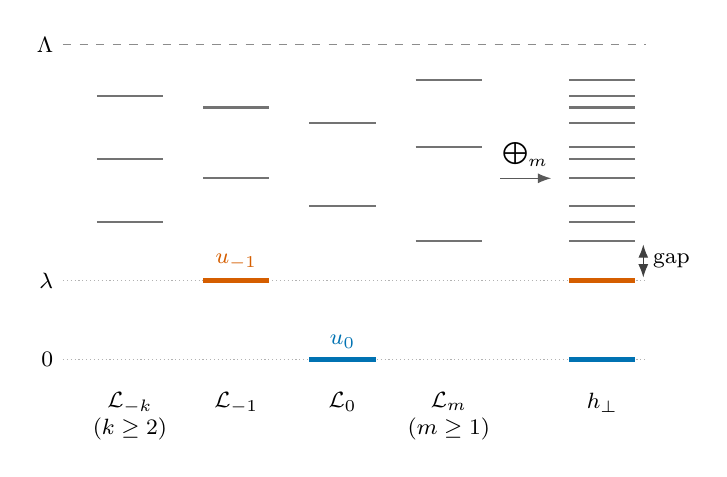
\begin{tikzpicture}[x=1cm,y=1cm,font=\footnotesize,>=Latex]
  \def\hw{0.42}
  % Reference lines at 0, lambda, and Lambda.
  \draw[black!30,densely dotted] (-0.25,0) -- (7.15,0);
  \draw[black!30,densely dotted] (-0.25,1) -- (7.15,1);
  \draw[black!45,dashed] (-0.25,4) -- (7.15,4);
  \node[anchor=east] at (-0.25,0) {$0$};
  \node[anchor=east] at (-0.25,1) {$\lambda$};
  \node[anchor=east] at (-0.25,4) {$\Lambda$};
  % Radial operators: excited and other-sector levels, all above lambda.
  \foreach \x/\levels in {0.6/{1.75,2.55,3.35},1.95/{2.3,3.2},
                          3.3/{1.95,3.0},4.65/{1.5,2.7,3.55}} {
    \foreach \y in \levels
      \draw[black!55,line width=0.8pt] (\x-\hw,\y) -- (\x+\hw,\y);
  }
  % Ground states of L_0 and L_{-1}.
  \draw[hkblue,line width=1.6pt] (3.3-\hw,0) -- (3.3+\hw,0);
  \node[anchor=south,text=hkblue] at (3.3,0.02) {$u_0$};
  \draw[hkorange,line width=1.6pt] (1.95-\hw,1) -- (1.95+\hw,1);
  \node[anchor=south,text=hkorange] at (1.95,1.02) {$u_{-1}$};
  % Union over sectors.
  \draw[->,black!65] (5.3,2.3) -- (5.95,2.3);
  \node[anchor=south] at (5.62,2.33) {$\bigoplus_m$};
  \foreach \y in {1.5,1.75,1.95,2.3,2.55,2.7,3.0,3.2,3.35,3.55}
    \draw[black!55,line width=0.8pt] (6.6-\hw,\y) -- (6.6+\hw,\y);
  \draw[hkblue,line width=1.6pt] (6.6-\hw,0) -- (6.6+\hw,0);
  \draw[hkorange,line width=1.6pt] (6.6-\hw,1) -- (6.6+\hw,1);
  \draw[<->,black!75] (7.12,1.04) -- (7.12,1.46);
  \node[anchor=west] at (7.12,1.25) {gap};
  % Column labels.
  \foreach \x/\lab in {0.6/{$\mathcal L_{-k}$\\$(k\ge2)$},
                       1.95/{$\mathcal L_{-1}$},
                       3.3/{$\mathcal L_0$},
                       4.65/{$\mathcal L_m$\\$(m\ge1)$},
                       6.6/{$h_\perp$}}
    \node[anchor=north,align=center] at (\x,-0.3) {\lab};
\end{tikzpicture}
% End embedded figure from planar-spectrum.tex
\space % Preserve spacing at the former input boundary.
 \caption{Spectral ordering in Lemma~\ref{lem:ordering}.
 The first four columns show schematic eigenvalues in angular
 sectors, and the final column combines them. The states $u_0$ and
 $u_{-1}$ give the simple eigenvalues $0$ and $\lambda$.
 All other eigenvalues lie above $\lambda$ by factorization in the
 sector $m=0$, ground-state simplicity in $m=-1$, and form comparison
 in the remaining sectors. Below $\Lambda$, eigenvalues are isolated
 and have finite multiplicity, giving a strict gap above $\lambda$.}
 \label{fig:planar-spectrum}
\end{figure}

\begin{proof}[Proof of Lemma~\ref{lem:ordering}]
We first show that $u_0$ and $u_{-1}$ are the ground states of
$\mathcal L_0$ and $\mathcal L_{-1}$, so that $\mathcal L_0\ge0$ and
$\mathcal L_{-1}\ge\lambda$. For $\mathcal L_0$ this follows from the
factorization, since $\ip{\phi}{\mathcal L_0\phi}=\|D\phi\|^2\ge0$ and
$\mathcal L_0u_0=0$. For $\mathcal L_{-1}$ we use the ground-state
representation with respect to the positive eigenfunction $u_{-1}$.
Writing $\phi=u_{-1}w$ with $\phi\in C_c^\infty(0,\infty)$ and
integrating by parts with $\mathcal L_{-1}u_{-1}=\lambda u_{-1}$ gives
\begin{equation*}
 \ip{\phi}{(\mathcal L_{-1}-\lambda)\phi}
   =\int_0^\infty u_{-1}^2|\partial_rw|^2\,r\,\mathrm{d}r\ge0.
\end{equation*}
Since $\mathcal L_{-1}$ is the Friedrichs realization,
$C_c^\infty(0,\infty)$ is a form core, and hence
$\mathcal L_{-1}\ge\lambda$. Both ground states are simple. For each
eigenvalue, the solutions of the radial equation that are regular at
$r=0$ form a one-dimensional space.

For $m\ge1$ and $k\ge2$, we have directly from Eq.~\eqref{eq:Lm}
\begin{align*}
 \mathcal L_m-\mathcal L_{-1}&=\frac{m^2-1+2(m+1)ra(r)}{r^2}>0,\\
 \mathcal L_{-k}-\mathcal L_{-1}&=\frac{(k-1)(k+1-2ra(r))}{r^2}>0.
\end{align*}
The first difference is positive because $m^2\ge1$ and $r a>0$, the
second because $k\ge2$ and $r a<1$. Let $n$ be $m$ or
$-k$. Since $\mathcal L_n-\mathcal L_{-1}$ is multiplication by a
positive function, the quadratic form of $\mathcal L_n$ dominates that
of $\mathcal L_{-1}$ on $C_c^\infty(0,\infty)$, so the form domain of
$\mathcal L_n$ is contained in that of $\mathcal L_{-1}$. Suppose that
$\mathcal L_n\psi=E\psi$ with $\|\psi\|=1$. Then
\begin{equation*}
 E=\ip{\psi}{\mathcal L_{-1}\psi}
   +\ip{\psi}{(\mathcal L_n-\mathcal L_{-1})\psi}>\lambda,
\end{equation*}
because $\mathcal L_{-1}\ge\lambda$ and the second term is the integral
of a positive function against $|\psi|^2$, which is strictly positive
for $\psi\ne0$. Hence every eigenvalue of $\mathcal L_m$ with
$m\ge1$ and of $\mathcal L_{-k}$ with $k\ge2$ is strictly greater
than $\lambda$.

It remains to exclude an excited eigenstate of $\mathcal L_0$ with
energy $E\le\lambda$. Let $\mathcal L_0\psi=E\psi$ with $\psi\ne0$ and
$\psi\perp u_0$. The kernel of $D$ consists of the solutions of
$\partial_r\psi+U_0\psi=0$, that is, of multiples of $u_0$. Hence
$\phi=D\psi\ne0$, and $E\|\psi\|^2=\ip{\psi}{D^*D\psi}=\|\phi\|^2>0$.
Moreover, $D^*\phi=\mathcal L_0\psi=E\psi$ lies in the domain of $D$, so
$\phi$ lies in the domain of $DD^*$ and
\begin{equation*}
 DD^*\phi=D(E\psi)=E\phi .
\end{equation*}
By Eq.~\eqref{eq:general-partner},
\begin{align*}
 E\|\phi\|^2=\ip{\phi}{\mathcal L_{-1}\phi}
   +2\int_0^\infty\left(\partial_rU_0+\frac {a(r)}{r}\right)|\phi|^2\,r\,\mathrm{d}r
   >\lambda\|\phi\|^2,
\end{align*}
because $\mathcal L_{-1}\ge\lambda$ and $\partial_rU_0+a/r>0$. Thus
$E>\lambda$, and every excited eigenvalue of $\mathcal L_0$ is strictly
greater than $\lambda$.

We now collect the sectors. The eigenvalue $0$ occurs only in the
sector $m=0$, as the simple ground state of $\mathcal L_0$, since all
other $\mathcal L_m$ are bounded below by $\lambda>0$. The eigenvalue
$\lambda$ occurs only in the sector $m=-1$, as the simple ground state
of $\mathcal L_{-1}$. Every other eigenvalue of every $\mathcal L_m$ is
strictly greater than $\lambda$. Since $\lambda<\Lambda$, the
spectrum of $h_\perp$ in $(-\infty,\lambda]$ consists of eigenvalues,
each of which is an eigenvalue of some $\mathcal L_m$. As multiplicities
add over sectors, $0$ and $\lambda$ are simple eigenvalues of
$h_\perp$, and $h_\perp$ has no other spectrum in
$(-\infty,\lambda]$. Infinitely many sectors could still produce
eigenvalues above $\lambda$ accumulating at $\lambda$. This is excluded
because the spectrum of $h_\perp$ below $\Lambda$ consists of isolated
eigenvalues of finite multiplicity. Hence there is an $\varepsilon>0$ such
that $h_\perp$ has no spectrum in $(\lambda,\lambda+\varepsilon)$, which is
the strict gap.
\end{proof}

Direct calculation using $\mathcal L_0u_0=0$ gives the differential
factorization identities in Eq.~\eqref{eq:general-partner}.
To apply them to eigenfunctions, we must also check that the operator
domains agree. In the constructions of Steps~3 and~4 of
Sec.~\ref{sec:noninteracting-proof}, $U_0$ is smooth and $O(r)$ at the origin.
The closure defining $D$ therefore requires finite radial kinetic
energy near $r=0$, but imposes no condition $\psi(0)=0$.
Smooth, compactly supported radial functions that are nonzero at the
origin can be approximated in the form norm (the graph norm of $D$)
by functions that vanish near zero. The closed form $\|D\psi\|^2$
identifies $D^*D$ with the Friedrichs realization of $\mathcal L_0$.
Among local eigenfunction solutions, this admits the regular branch
and excludes the $\log r$ branch, whose kinetic energy diverges.
The operator $DD^*$ has the centrifugal term $1/r^2$, with local
solutions having leading behaviors $r$ and $1/r$. The latter is not
in $L^2(r\,\mathrm{d}r)$ near zero, so no boundary condition is needed there.
No boundary condition is needed at infinity either, since the radial
potentials in these examples grow quadratically or approach a finite
constant. The corresponding differential expression consequently has
a unique self-adjoint realization. Since $DD^*$ is self-adjoint,
uniqueness shows that the two sides of the factorization have the
same action and the same domain.

\section{The Dirac monopole Hamiltonian}
\label{app:monopole}

This appendix collects the definitions and spectral properties
of the monopole Hamiltonians used in Sec.~\ref{sec:monopole} and in
the proof of Theorem~\ref{thm:monopole}.

\subsection{Connections, sections, and the Hamiltonian}
\label{app:monopole-definitions}

We use spherical coordinates $(s,\vartheta,\varphi)$,
where $s=|\mathbf x|$ and
$\widehat{\mathbf x}=\mathbf x/s$ denotes the unit radial vector.
For $g=\pm\tfrac12$ set
\begin{equation}
 \begin{aligned}
 \B_g(\mathbf x)&=g\frac{\mathbf x}{|\mathbf x|^3},\\
 \A_g^{\mathrm N}&=\frac{g(1-\cos\vartheta)}{s\sin\vartheta}\mathbf e_\varphi,\\
 \A_g^{\mathrm S}&=-\frac{g(1+\cos\vartheta)}{s\sin\vartheta}\mathbf e_\varphi.
 \end{aligned}
 \label{eq:monopole-gauges}
\end{equation}
The north potential is used away from the negative $z$ axis, and the
south potential away from the positive $z$ axis, with the origin
excluded throughout. Both are smooth on their respective domains
and have curl $\B_g$. On the overlap,
\begin{equation}
 \A_g^{\mathrm N}-\A_g^{\mathrm S}=\nabla(2g\varphi),\qquad
 \psi^{\mathrm N}=e^{-2\mathrm{i}g\varphi}\psi^{\mathrm S}.
 \label{eq:transition}
\end{equation}
Following Wu and Yang \cite{WuYang1976}, we represent each wavefunction
by local functions $\psi^{\mathrm N}$ and $\psi^{\mathrm S}$ on the two
patches. On their overlap, these functions are related by the phase
factor in Eq.~\eqref{eq:transition}, whose sign follows from our
convention $-\mathrm{i}\nabla+\A$ in Sec.~\ref{sec:preliminaries}.
The two local functions therefore represent a single wavefunction,
with their values on the overlap related by the prescribed gauge
phase. Such a wavefunction is called a section of the monopole
line bundle. Write $\A_g$ for the connection
given by the pair $(\A_g^{\mathrm N},\A_g^{\mathrm S})$, and $\bpi_g=-\mathrm{i}\nabla+\A_g$ for its
covariant momentum. Figure~\ref{fig:monopole} shows the two fields and
the two patches.

\begin{figure}[t]
 \centering
% Begin embedded figure from monopole-patches.tex
% Monopole fields and patches; the z axis is vertical.
% Requires TikZ library arrows.meta and colors hkblue/hkorange from the preamble.
% Top row: field lines of B_g for g=+1/2 (outward) and g=-1/2 (inward) in a
% plane containing the z axis; the dashed circle is a sphere about the origin.
% Bottom row: the north patch (theta<pi) and south patch (theta>0) on such a
% sphere, viewed from slightly above. The omitted pole is hollow, and the
% dashed half-axis through it is where that patch potential is singular.
\pgfdeclareradialshading{patchN}{\pgfpoint{-14bp}{14bp}}
  {color(0bp)=(white); color(72bp)=(hkblue!32)}
\pgfdeclareradialshading{patchS}{\pgfpoint{-14bp}{14bp}}
  {color(0bp)=(white); color(72bp)=(hkorange!32)}
\begin{tikzpicture}[x=1cm,y=1cm,font=\footnotesize,>=Latex]
  \tikzset{tip/.style={-{Latex[length=1.6mm,width=1.3mm]}}}
  % Fields.
  \foreach \cx/\sgn/\panel/\qlabel/\flux in
    {0/1/a/{+\tfrac12}/{+2\pi},4/-1/b/{-\tfrac12}/{-2\pi}} {
    \begin{scope}[shift={(\cx,0)}]
      \draw[black!30,dashed,line width=0.4pt] (0,0) circle[radius=0.95];
      \foreach \ang in {22.5,67.5,...,337.5} {
        \ifnum\sgn=1
          \draw[black!75,line width=0.5pt,tip] (\ang:0.22) -- (\ang:0.75);
          \draw[black!75,line width=0.5pt] (\ang:0.7) -- (\ang:1.25);
        \else
          \draw[black!75,line width=0.5pt,tip] (\ang:1.25) -- (\ang:0.55);
          \draw[black!75,line width=0.5pt] (\ang:0.6) -- (\ang:0.22);
        \fi
      }
      \filldraw[fill=white,draw=black,line width=0.6pt] (0,0) circle[radius=0.13];
      \draw[line width=0.6pt] (-0.07,0) -- (0.07,0);
      \ifnum\sgn=1
        \draw[line width=0.6pt] (0,-0.07) -- (0,0.07);
      \fi
      \node[font=\small] at (0,1.6) {(\panel)\quad$g=\qlabel$};
      \node at (0,-1.55) {flux $\flux$};
    \end{scope}
  }
  % Patches on a sphere of radius 0.95, viewed from elevation arcsin(1/4):
  % the equator is an ellipse with semi-axes 0.95, 0.24, and the poles
  % sit at height +-0.92.
  \foreach \cx/\col/\dir/\panel/\name/\pot/\range in
    {0/hkblue/-1/c/north/N/{0\le\vartheta<\pi},
     4/hkorange/1/d/south/S/{0<\vartheta\le\pi}} {
    \begin{scope}[shift={(\cx,-3.95)}]
      \shade[shading=patch\pot] (0,0) circle[radius=0.95];
      \draw[black!55,line width=0.5pt] (0,0) circle[radius=0.95];
      \draw[black!30,densely dashed,line width=0.4pt]
        (0.95,0) arc[start angle=0,end angle=180,x radius=0.95,y radius=0.24];
      \draw[black!50,line width=0.4pt]
        (-0.95,0) arc[start angle=180,end angle=360,x radius=0.95,y radius=0.24];
      % Omitted half-axis, seen through the sphere inside it.
      \draw[\col!55,densely dashed,line width=0.6pt] (0,0) -- (0,0.92*\dir);
      \draw[\col,densely dashed,line width=0.9pt] (0,0.92*\dir) -- (0,1.35*\dir);
      \fill[black!70] (0,0) circle[radius=0.035];
      % Included and omitted poles.
      \fill[black!70] (0,-0.92*\dir) circle[radius=0.04];
      \filldraw[fill=white,draw=\col,line width=0.7pt] (0,0.92*\dir) circle[radius=0.065];
      \node[text=\col!80!black] at (0.42,-0.5*\dir) {$\A_g^{\mathrm \pot}$};
      \node[font=\small] at (0,1.7) {(\panel)\quad\name\ patch};
      \node at (0,-1.7) {$\range$};
    \end{scope}
  }
\end{tikzpicture}
% End embedded figure from monopole-patches.tex
\space % Preserve spacing at the former input boundary.
 \caption{Monopole fields and patches of Theorem~\ref{thm:monopole},
 with the $z$ axis vertical. (a),(b) Field lines of $\B_g$ for
 $g=\pm\tfrac12$. The flux through every sphere about the origin
 (dashed) is $4\pi g=\pm2\pi$. (c),(d) The north and south patches,
 on which $\A_g^{\mathrm N}$ and $\A_g^{\mathrm S}$ are regular, drawn
 on a sphere about the origin. Each omits one pole (open circle) and,
 in $\R^3_*$, the half-axis through it (dashed).}
 \label{fig:monopole}
\end{figure}

Put $\R^3_*=\R^3\setminus\{0\}$ and denote the north and south patches
by $U_{\mathrm N}$ and $U_{\mathrm S}$, respectively. The one-particle
space of square-integrable sections is
\begin{equation*}
 \cH_g=\bigl\{
 (\psi^{\mathrm N},\psi^{\mathrm S})
 \in L^2(U_{\mathrm N})\times L^2(U_{\mathrm S})
 \bigm|\;
 \psi^{\mathrm N}=e^{-2\mathrm{i}g\varphi}\psi^{\mathrm S}
 \text{ a.e. on }U_{\mathrm N}\cap U_{\mathrm S}
 \bigr\}.
\end{equation*}
For $\psi=(\psi^{\mathrm N},\psi^{\mathrm S})\in\cH_g$, the norm is
\begin{equation*}
 \|\psi\|_{\cH_g}^2
 =\int_{\R^3_*}|\psi(\mathbf x)|^2\,\mathrm{d}\mathbf x,
\end{equation*}
where $|\psi|^2$ is computed using either local representative on its
patch. The phase relation in Eq.~\eqref{eq:transition} ensures that
the two expressions agree on the overlap. Define
\begin{equation}
 \begin{aligned}
 h^{v,\A_g}&=\bpi_g^2+v,\qquad v(\mathbf x)=s^2,\\
 H^{v,\A_g}&=h^{v,\A_g}_1+h^{v,\A_g}_2+W
       \quad\text{on }\bigwedge\nolimits^2\cH_g,
 \end{aligned}
 \label{eq:monopole-H}
\end{equation}
with $W=|\mathbf x_1-\mathbf x_2|^{-1}$. This is
Eq.~\eqref{eq:Hamiltonian} with $\kappa=1$, the vector potential
replaced by the connection $\A_g$, and $L^2(\R^3)$ replaced by $\cH_g$.
We always use the Friedrichs realization of $H^{v,\A_g}$. Let
$\mathcal D_g\subset\bigwedge^2\cH_g$ consist of the antisymmetric
smooth sections with compact support in $\R^3_*\times\R^3_*$. For
$\Psi\in\mathcal D_g$,
\begin{equation}
 \ip{\Psi}{H^{v,\A_g}\Psi}
   =\sum_{i=1}^2\Bigl(\|\bpi_{g,i}\Psi\|_2^2
   +\bigl\||\mathbf x_i|\Psi\bigr\|_2^2\Bigr)
   +\ip{\Psi}{W\Psi}\ge0,
 \label{eq:monopole-form}
\end{equation}
where $\bpi_{g,i}$ acts on $\mathbf x_i$. This nonnegative form is
closable, and $H^{v,\A_g}$ denotes the self-adjoint operator associated
with its closure \cite[Theorem~X.23]{RS2}. A choice is needed because even
the one-particle operator $h^{v,\A_g}$ is not essentially self-adjoint
on smooth sections with compact support in $\R^3_*$. The Friedrichs
realization fixes the behavior at the monopole in the lowest angular
sector, as specified by Eq.~\eqref{eq:friedrichs-bc} in
Appendix~\ref{app:monopole-domains}.


The density and total current defined in Sec.~\ref{sec:preliminaries}
are calculated separately on each patch. Gauge invariance ensures that the two
calculations give the same values wherever the patches overlap.
They therefore define a single particle density and a single
total-current density throughout $\R^3\setminus\{0\}$.

\subsection{Radial reduction, Friedrichs realization, and free spectrum}
\label{sec:monopole-spectrum}
\label{app:monopole-domains}

The covariant angular momentum $\mathbf L_g$ and the radial splitting
of the kinetic energy are
\begin{equation}
 \mathbf L_g=\mathbf x\times\bpi_g+g\frac{\mathbf x}{s},\qquad
 \bpi_g^2=-\partial_s^2-\frac2s\partial_s
                   +\frac{\mathbf L_g^2-g^2}{s^2}.
 \label{eq:radial-splitting}
\end{equation}
The eigenvalues of $\mathbf L_g^2$ are $j(j+1)$ with
$j=|g|,|g|+1,\ldots$, and the angular sector $j$ has dimension $2j+1$.
Thus the $j=\tfrac12$ sector is a \emph{doublet}, with
angular-momentum projections $m=\pm\tfrac12$.
A two-particle state with total angular momentum zero is
called a \emph{singlet} and is invariant under simultaneous
rotations of both particles. These terms describe angular
momentum in the monopole field. The particles themselves
are spinless.

For fixed $j$, put
\begin{equation}
 \ell_j=\frac{\sqrt{(2j+1)^2-4g^2}-1}{2}.
\end{equation}
Then $\ell_j(\ell_j+1)=j(j+1)-g^2$.
For $\psi=s^{-1}u(s)Y$, where $Y$ is normalized on the unit
sphere and satisfies $\mathbf L_g^2Y=j(j+1)Y$, the spherical
volume element gives $\|\psi\|_2=\|u\|_{L^2(0,\infty)}$.
Equation~\eqref{eq:radial-splitting} then yields
$h^{v,\A_g}\psi=s^{-1}(\tau_j u)Y$,
where
\begin{equation}
 \tau_j=-\frac{\mathrm{d}^2}{\mathrm{d}s^2}+\frac{\ell_j(\ell_j+1)}{s^2}+s^2.
 \label{eq:monopole-radial}
\end{equation}

The following lemma establishes the boundary condition at the
monopole, the free spectrum, and the form-domain and compactness
properties needed for the interacting spectral comparison.

\begin{lemma}[Monopole domains and compactness]
\label{lem:monopole-domains}
For $g=\pm\tfrac12$ and $v(\mathbf x)=|\mathbf x|^2$, the
Friedrichs realization of $h^{v,\A_g}$ selects the regular branch
$s^{\ell_j+1}$ for radial eigenfunctions at the origin and has
compact resolvent. Coulomb repulsion $W$ is infinitesimally form
bounded with respect to the noninteracting two-particle oscillator
form. The free and interacting two-particle Hamiltonians therefore
have the same form domain and both have compact resolvent.
\end{lemma}

\begin{proof}
Near $s=0$, two independent solutions of $\tau_j u=\lambda u$
have leading behaviors $s^{\ell_j+1}$ and $s^{-\ell_j}$.
Both are square integrable with respect to the radial measure
$\mathrm{d}s$ exactly when $\ell_j<\tfrac12$, equivalently
$\ell_j(\ell_j+1)<\tfrac34$.
Square integrability alone then allows both behaviors, so a
boundary condition at the origin is needed to specify a
self-adjoint radial operator. This is the \emph{limit-circle}
case \cite[pp.~159--161]{RS2}.
For $\ell_j\ge\tfrac12$, only the first behavior is square
integrable, and no additional boundary condition is needed
at the origin. This is the \emph{limit-point} case.

For $|g|=\tfrac12$, the coefficient
$\ell_j(\ell_j+1)=j(j+1)-\tfrac14$ equals $\tfrac12$ when
$j=\tfrac12$ and is at least $\tfrac72$ when $j\ge\tfrac32$.
Thus only the $j=\tfrac12$ sector, where
$\ell_{1/2}=(\sqrt3-1)/2$, lies below the limit-circle threshold
$\tfrac34$. At infinity, the harmonic term gives one Gaussian-decaying
and one Gaussian-growing solution, up to algebraic factors.
Only the decaying solution is square integrable there, so every
$\tau_j$ is limit point at infinity.
Each of the two angular components $m=\pm\tfrac12$ in the lowest
sector contributes deficiency indices $(1,1)$, since the origin is
limit circle and infinity is limit point. All higher angular sectors
contribute $(0,0)$, since both endpoints are limit point
\cite[Sec.~9.2]{Teschl2009}. Thus the closure of the one-particle
operator initially defined on smooth sections with compact support
in $\R^3_*$ has deficiency indices $(2,2)$. Its self-adjoint extensions
differ through boundary conditions at the monopole in this doublet.
(Boundary conditions of this kind also arise for the Pauli
\cite{KarSch1997} and Dirac \cite{KYG1977} Hamiltonians in a monopole
field.) The Friedrichs
realization selects the principal solution $s^{\ell_{1/2}+1}$
\cite{Kalf1978,NZ1992}. In the $j=\tfrac12$ sector, its operator
domain consists of those $u$ for which $u,u'$ are locally absolutely
continuous on $(0,\infty)$, $u,\tau_{1/2}u\in L^2(0,\infty)$, and
\begin{equation}
 \lim_{s\to0}\bigl(s^{\ell_{1/2}+1}u'(s)
   -(\ell_{1/2}+1)s^{\ell_{1/2}}u(s)\bigr)=0.
 \label{eq:friedrichs-bc}
\end{equation}
This excludes $u\sim s^{-\ell_{1/2}}$, which has infinite form
$\int_0^1\bigl(|u'|^2+\ell_{1/2}(\ell_{1/2}+1)s^{-2}|u|^2\bigr)\,\mathrm{d}s$.
With this boundary choice, radial oscillator separation gives the
eigenvalues of the Friedrichs realization of the one-particle
Hamiltonian $h^{v,\A_g}$, for $n=0,1,\ldots$,
\begin{equation}
 \varepsilon_{n,j}=4n+2+\sqrt{(2j+1)^2-4g^2}.
 \label{eq:one-particle-spectrum}
\end{equation}
For any normalized angular eigenfunction $Y$ satisfying
$\mathbf L_g^2Y=j(j+1)Y$, the corresponding one-particle eigenfunctions
have the separated form
\begin{equation*}
 \begin{aligned}
 \psi(s,\widehat{\mathbf x})
   &=s^{-1}u_{n,j}(s)Y(\widehat{\mathbf x}),\\
 u_{n,j}(s)
   &=C_{n,j}s^{\ell_j+1}e^{-s^2/2}L_n^{\ell_j+1/2}(s^2).
 \end{aligned}
\end{equation*}
Here $L_n^\alpha$ denotes a generalized Laguerre polynomial and
$C_{n,j}$ is chosen so that $\|u_{n,j}\|_{L^2(0,\infty)}=1$.
These functions satisfy $\tau_j u_{n,j}=\varepsilon_{n,j}u_{n,j}$
and $h^{v,\A_g}\psi=\varepsilon_{n,j}\psi$.
For $n=0$, $L_0^\alpha=1$, so the radial factor $u_{0,j}/s$ is
proportional to $s^{\ell_j}e^{-s^2/2}$, with energy $2\ell_j+3$.
The form of $u_{0,j}$ is suggested by combining the regular behavior
$s^{\ell_j+1}$ at the origin with the Gaussian decay $e^{-s^2/2}$.
Direct differentiation gives
\begin{equation*}
 \frac{u_{0,j}''}{u_{0,j}}
 =\frac{\ell_j(\ell_j+1)}{s^2}+s^2-(2\ell_j+3),
\end{equation*}
so substitution into Eq.~\eqref{eq:monopole-radial} yields
$\tau_j u_{0,j}=(2\ell_j+3)u_{0,j}$.

These eigenvalues have finite
multiplicity and tend to infinity as $n$ or $j$ tends to infinity.
Thus $h^{v,\A_g}$ and the noninteracting two-particle oscillator
have compact resolvent.

The Coulomb singularity is controlled on the magnetic form domain.
The diamagnetic inequality for sections applies to the globally
defined scalar modulus $|\Psi|$. The Hardy inequality in the relative
coordinate therefore gives
\begin{equation}
 \int\frac{|\Psi|^2}{|\mathbf x_1-\mathbf x_2|^2}
    \,\mathrm{d}\mathbf x_1\,\mathrm{d}\mathbf x_2
    \le2\sum_{i=1}^2\|\bpi_{g,i}\Psi\|_2^2.
 \label{eq:Hardy}
\end{equation}
Consequently, with $T_g[\Psi]=\sum_i\|\bpi_{g,i}\Psi\|_2^2$,
\begin{equation}
 \ip{\Psi}{W\Psi}
   \le\sqrt2\|\Psi\|_2\sqrt{T_g[\Psi]}
   \le\delta T_g[\Psi]+\frac1{2\delta}\|\Psi\|_2^2.
\end{equation}
Thus Coulomb repulsion is infinitesimally form bounded, and the
interacting form has the same domain as the free oscillator form.
In particular, adding Coulomb repulsion preserves the Friedrichs
form-domain choice at the monopole for each particle. The free and
interacting forms have equivalent form norms, so the compact
embedding of the free form domain is preserved. Hence the
interacting Hamiltonian also has compact resolvent.
\end{proof}

\begin{thebibliography}{99}

\bibitem{HK1964}
P. Hohenberg and W. Kohn,
Inhomogeneous electron gas,
\href{https://doi.org/10.1103/PhysRev.136.B864}
{Phys. Rev. \textbf{136}, B864 (1964)}.

\bibitem{CV2002}
K. Capelle and G. Vignale,
Nonuniqueness and derivative discontinuities in density-functional
theories for current-carrying and superconducting systems,
\href{https://doi.org/10.1103/PhysRevB.65.113106}
{Phys. Rev. B \textbf{65}, 113106 (2002)}.

\bibitem{LB2014}
A. Laestadius and M. Benedicks,
Hohenberg--Kohn theorems in the presence of magnetic field,
\href{https://doi.org/10.1002/qua.24668}
{Int. J. Quantum Chem. \textbf{114}, 782 (2014)}.

\bibitem{VR1987}
G. Vignale and M. Rasolt,
Density-functional theory in strong magnetic fields,
\href{https://doi.org/10.1103/PhysRevLett.59.2360}
{Phys. Rev. Lett. \textbf{59}, 2360 (1987)}.

\bibitem{LT2018}
A. Laestadius and E. I. Tellgren,
Density--wave-function mapping in degenerate current-density-functional
theory,
\href{https://doi.org/10.1103/PhysRevA.97.022514}
{Phys. Rev. A \textbf{97}, 022514 (2018)}.

\bibitem{Diener1991}
G. Diener,
Current-density-functional theory for a non-relativistic electron gas
in a strong magnetic field,
\href{https://doi.org/10.1088/0953-8984/3/47/014}
{J. Phys.: Condens. Matter \textbf{3}, 9417 (1991)}.

\bibitem{PS2010}
X.-Y. Pan and V. Sahni,
Density and physical current density functional theory,
\href{https://doi.org/10.1002/qua.22862}
{Int. J. Quantum Chem. \textbf{110}, 2833 (2010)}.

\bibitem{Tellgren2012}
E. I. Tellgren, S. Kvaal, E. Sagvolden, U. Ekstr\"om,
A. M. Teale, and T. Helgaker,
Choice of basic variables in current-density-functional theory,
\href{https://doi.org/10.1103/PhysRevA.86.062506}
{Phys. Rev. A \textbf{86}, 062506 (2012)}.

\bibitem{LB2015}
A. Laestadius and M. Benedicks,
Nonexistence of a Hohenberg--Kohn variational principle in total
current-density-functional theory,
\href{https://doi.org/10.1103/PhysRevA.91.032508}
{Phys. Rev. A \textbf{91}, 032508 (2015)}.

\bibitem{VUC2013}
G. Vignale, C. A. Ullrich, and K. Capelle,
Comment on ``Density and physical current density functional theory''
by Xiao-Yin Pan and Viraht Sahni,
\href{https://doi.org/10.1002/qua.24327}
{Int. J. Quantum Chem. \textbf{113}, 1422 (2013)}.

\bibitem{LPT2021}
A. Laestadius, M. Penz, and E. I. Tellgren,
Revisiting density-functional theory of the total current density,
\href{https://doi.org/10.1088/1361-648X/abf784}
{J. Phys.: Condens. Matter \textbf{33}, 295504 (2021)}.

\bibitem{Penz2023}
M. Penz, E. I. Tellgren, M. A. Csirik, M. Ruggenthaler, and
A. Laestadius,
The structure of the density-potential mapping. Part II: Including
magnetic fields,
\href{https://doi.org/10.1021/acsphyschemau.3c00006}
{ACS Phys. Chem. Au \textbf{3}, 492 (2023)}.

\bibitem{KS1965}
W. Kohn and L. J. Sham,
Self-consistent equations including exchange and correlation effects,
\href{https://doi.org/10.1103/PhysRev.140.A1133}
{Phys. Rev. \textbf{140}, A1133 (1965)}.

\bibitem{VR1988}
G. Vignale and M. Rasolt,
Current- and spin-density-functional theory for inhomogeneous
electronic systems in strong magnetic fields,
\href{https://doi.org/10.1103/PhysRevB.37.10685}
{Phys. Rev. B \textbf{37}, 10685 (1988)}.

\bibitem{Dirac1931}
P. A. M. Dirac,
Quantised singularities in the electromagnetic field,
\href{https://doi.org/10.1098/rspa.1931.0130}
{Proc. R. Soc. Lond. A \textbf{133}, 60 (1931)}.

\bibitem{Laestadius2014}
A. Laestadius,
Density functionals in the presence of magnetic field,
\href{https://doi.org/10.1002/qua.24707}
{Int. J. Quantum Chem. \textbf{114}, 1445 (2014)}.

\bibitem{Laestadius2019}
A. Laestadius, E. I. Tellgren, M. Penz, M. Ruggenthaler,
S. Kvaal, and T. Helgaker,
Kohn--Sham theory with paramagnetic currents: Compatibility and
functional differentiability,
\href{https://doi.org/10.1021/acs.jctc.9b00141}
{J. Chem. Theory Comput. \textbf{15}, 4003 (2019)}.

\bibitem{Lieb1983}
E. H. Lieb,
Density functionals for Coulomb systems,
\href{https://doi.org/10.1002/qua.560240302}
{Int. J. Quantum Chem. \textbf{24}, 243 (1983)}.

\bibitem{GT2001}
D. Gilbarg and N. S. Trudinger,
\href{https://doi.org/10.1007/978-3-642-61798-0}
{\emph{Elliptic Partial Differential Equations of Second Order}},
Classics in Mathematics (Springer, Berlin, 2001).

\bibitem{Garrigue2020}
L. Garrigue,
Unique continuation for many-body Schr\"odinger operators and the
Hohenberg--Kohn theorem. II. The Pauli Hamiltonian,
\href{https://doi.org/10.4171/DM/765}
{Doc. Math. \textbf{25}, 869 (2020)}.

\bibitem{WuYang1976}
T. T. Wu and C. N. Yang,
Dirac monopole without strings: Monopole harmonics,
\href{https://doi.org/10.1016/0550-3213(76)90143-7}
{Nucl. Phys. B \textbf{107}, 365 (1976)}.

\bibitem{GS2020}
S. J. Gustafson and I. M. Sigal,
\href{https://doi.org/10.1007/978-3-030-59562-3}
{\emph{Mathematical Concepts of Quantum Mechanics}},
3rd ed. (Springer, Cham, 2020).

\bibitem{Ichinose1978}
T. Ichinose,
Spectral properties of tensor products of linear operators. I,
\href{https://doi.org/10.1090/S0002-9947-1978-0472915-2}
{Trans. Amer. Math. Soc. \textbf{235}, 75 (1978)}.

\bibitem{Hall2015}
B. C. Hall,
\href{https://doi.org/10.1007/978-3-319-13467-3}
{\emph{Lie Groups, Lie Algebras, and Representations:
An Elementary Introduction}},
2nd ed., Graduate Texts in Mathematics, Vol.~222
(Springer, Cham, 2015).

\bibitem{RS2}
M. Reed and B. Simon,
\emph{Methods of Modern Mathematical Physics II: Fourier Analysis,
Self-Adjointness} (Academic Press, New York, 1975).

\bibitem{Teschl2009}
G. Teschl,
\href{https://www.mat.univie.ac.at/~gerald/ftp/book-schroe/schroe.pdf}
{\emph{Mathematical Methods in Quantum Mechanics:
With Applications to Schr\"odinger Operators}},
Graduate Studies in Mathematics, Vol.~99
(American Mathematical Society, Providence, RI, 2009).

\bibitem{KarSch1997}
E. Karat and M. Schulz,
Self-adjoint extensions of the Pauli equation in the presence of a
magnetic monopole,
\href{https://doi.org/10.1006/aphy.1996.5638}
{Ann. Phys. (N.Y.) \textbf{254}, 11 (1997)}.

\bibitem{KYG1977}
Y. Kazama, C. N. Yang, and A. S. Goldhaber,
Scattering of a Dirac particle with charge $Ze$ by a fixed magnetic
monopole,
\href{https://doi.org/10.1103/PhysRevD.15.2287}
{Phys. Rev. D \textbf{15}, 2287 (1977)}.

\bibitem{Kalf1978}
H. Kalf,
A characterization of the Friedrichs extension of Sturm--Liouville
operators,
\href{https://doi.org/10.1112/jlms/s2-17.3.511}
{J. London Math. Soc. (2) \textbf{17}, 511 (1978)}.

\bibitem{NZ1992}
H.-D. Niessen and A. Zettl,
Singular Sturm--Liouville problems: The Friedrichs extension and
comparison of eigenvalues,
\href{https://doi.org/10.1112/plms/s3-64.3.545}
{Proc. London Math. Soc. (3) \textbf{64}, 545 (1992)}.

\end{thebibliography}
\end{document}
